%!TEX root = ../tese.tex
%!TEX encoding = UTF-8 Unicode
\section{Overhead}\label{sec:eval:peformance}

The performance evaluation aims to prove Shuttle scalability and capability to support small and enterprise applications (Section \ref{sec:eval:test_description}). Its results should match the evaluation metrics bounds that allow to use Shuttle in real environments. We evaluate Shuttle's performance considering the throughput of the application, the size of the logs and the recovery time. We also estimate the cost of deployment of Shuttle on a public cloud provider (AWS \cite{aws}). \\

We run Shuttle in \acf{AWS}. All instances are connected by gigabit ethernet (780Mbps measured with \emph{iperf}, 0.176ms round-trip time measured with \emph{ping}) and have the \emph{Java 1.7 HotSpot} 64-Bit Server \ac{VM} version installed. Even when the \ac{JVM} performance increases as the bytecode is compiled by the \ac{JIT} compiler, we run every test on new \ac{JVM} instances. They have a 32GB local general purpose \ac{SSD}. We used the local \ac{SSD} since its performance on read is better than a 500 Provisioned \ac{IOPS} \ac{SSD} of 25GB \ref{tab:disk_throughput}. We allocated 5GB of heap to the \ac{JVM} and we disabled database replication (each data item is stored in one data node). \hl{o sistema de replicacao de base de dados foi desactivado}

\begin{table}[ht]
\centering
\begin{tabular}{l|rrrrr}
                   & \multicolumn{1}{l}{\textbf{putc()}} & \multicolumn{1}{l}{\textbf{Block Write}} & \multicolumn{1}{l}{\textbf{Create,Change,Rewrite}} & \multicolumn{1}{l}{\textbf{getc()}} & \multicolumn{1}{l}{\textbf{Block Read}}  \\ \hline
\textbf{EBS SSD}      & 631                                 & 83264                                    & 44448                                              & 1562                                & 105723                                  \\
\textbf{Local SSD} & 619                                 & 106546                                   & 186204                                             & 1577                                & 614790                                 
\end{tabular}
\caption[Comparison between a EBS Provisioned IOPS (SSD) and local SSD instance]{Comparison between a EBS Provisioned IOPS (SSD), which supports up to 500 IOPS, and a local SSD instance using bonnie++ (KB/s)}
\label{tab:disk_throughput}
\end{table}




%%%%%%%%%%%%%%%%%%%%%%%%%%%%%%%%%%%%%%%%%%%%%%%%%%%%%%%%%%%%%%%%%%%%%%%%%%%%%%%%%%%%%%%%%%%%%%%%%%%%%%%%%%%%%%%%
\subsection{Performance Overhead}\label{sec:eval:performance}
In this section, we quantify the overhead imposed by each component of Shuttle.

\subsubsection{Database}\label{sec:eval:performance:database}
We measured the overhead of Shuttle on database instances. We expected it to be the major impact of Shuttle because Shuttle logs every operation. We used \acf{YCSB} \cite{ycsb}. \ac{YCSB} was developed to measure the performance of the new generation of cloud data serving systems, such as Voldemort used in Shuttle. We extended \ac{YCSB} to support the latest version of Voldemort and to use \acf{protobuf} as request format.\\

We used 6 \textit{m3.large} instances (7 \ac{ECU}s, 2 vCPUs, 2.8 GHz, Intel Xeon E5-2680v2, 3.75 GiB memory, 2 x 16 GiB Storage Capacity) to run each database node. The database service was accessed by two \textit{c3.xlarge} instances (14 \ac{ECU}s, 4 vCPUs, 2.8 GHz, Intel Xeon E5-2680v2, 7.5 GB of memory, 2 x 40 GB Storage Capacity).\\


We ran 4 out of 5 workloads (Table \ref{tab:workload_description}) proposed \emph{in} \cite{ycsb}. Workload E (Short ranges) is not supported by Voldemort. \hl{deixei apenas na tabela, iria estar a ler a tabela...} Our database consisted of 60 million 1KB record (total database size: 60GB). Each instance thus had an average of 10GB of data, more than it could cache entirely in memory. Read operations retrieve entire records, while update operations modify one of the ten record fields \cite{ycsb}.

\begin{table}[ht]
\centering
\begin{tabular}{p{0.18\linewidth}p{0.15\linewidth}p{0.09\linewidth}p{0.48\linewidth}}
\textbf{Workload}       & \textbf{Operations}                   & \textbf{Key \newline Selection} & \textbf{Application Example} \\ \hline
A - Update heavy        & Read: 50\% \newline Update: 50\%               & Zipfian                & Session store recording recent actions\\ \hline
B - Read mostly         & Read: 95\% \newline Update: 5\%                & Zipfian                & Photo tagging; add a tag is an update, but most operations are to read tags\\ \hline
C - Read only           & Read: 100\%                           & Zipfian                & User profile cache, where profiles are constructed elsewhere (e.g., Hadoop)\\ \hline
D - Read latest         & Read: 95\% \newline Insert: 5\%                & Latest                 & User status updates; people want to read the latest \\ \hline
% F - Read-modify-write  & Get: 50\%  \newline Read-modify-write: 50\%    & Zipfian                & User database, where user records are read and modified by the user or to record user activity.\\ \hline

\end{tabular}
\caption{Workload description}
\label{tab:workload_description}
\end{table}


\begin{figure}[!htb]
  \centering
  \subfloat[][\textbf{Workload A:} read operations]{\resizebox{0.45\linewidth}{!}{% GNUPLOT: LaTeX picture with Postscript
\begingroup
  \makeatletter
  \providecommand\color[2][]{%
    \GenericError{(gnuplot) \space\space\space\@spaces}{%
      Package color not loaded in conjunction with
      terminal option `colourtext'%
    }{See the gnuplot documentation for explanation.%
    }{Either use 'blacktext' in gnuplot or load the package
      color.sty in LaTeX.}%
    \renewcommand\color[2][]{}%
  }%
  \providecommand\includegraphics[2][]{%
    \GenericError{(gnuplot) \space\space\space\@spaces}{%
      Package graphicx or graphics not loaded%
    }{See the gnuplot documentation for explanation.%
    }{The gnuplot epslatex terminal needs graphicx.sty or graphics.sty.}%
    \renewcommand\includegraphics[2][]{}%
  }%
  \providecommand\rotatebox[2]{#2}%
  \@ifundefined{ifGPcolor}{%
    \newif\ifGPcolor
    \GPcolorfalse
  }{}%
  \@ifundefined{ifGPblacktext}{%
    \newif\ifGPblacktext
    \GPblacktexttrue
  }{}%
  % define a \g@addto@macro without @ in the name:
  \let\gplgaddtomacro\g@addto@macro
  % define empty templates for all commands taking text:
  \gdef\gplbacktext{}%
  \gdef\gplfronttext{}%
  \makeatother
  \ifGPblacktext
    % no textcolor at all
    \def\colorrgb#1{}%
    \def\colorgray#1{}%
  \else
    % gray or color?
    \ifGPcolor
      \def\colorrgb#1{\color[rgb]{#1}}%
      \def\colorgray#1{\color[gray]{#1}}%
      \expandafter\def\csname LTw\endcsname{\color{white}}%
      \expandafter\def\csname LTb\endcsname{\color{black}}%
      \expandafter\def\csname LTa\endcsname{\color{black}}%
      \expandafter\def\csname LT0\endcsname{\color[rgb]{1,0,0}}%
      \expandafter\def\csname LT1\endcsname{\color[rgb]{0,1,0}}%
      \expandafter\def\csname LT2\endcsname{\color[rgb]{0,0,1}}%
      \expandafter\def\csname LT3\endcsname{\color[rgb]{1,0,1}}%
      \expandafter\def\csname LT4\endcsname{\color[rgb]{0,1,1}}%
      \expandafter\def\csname LT5\endcsname{\color[rgb]{1,1,0}}%
      \expandafter\def\csname LT6\endcsname{\color[rgb]{0,0,0}}%
      \expandafter\def\csname LT7\endcsname{\color[rgb]{1,0.3,0}}%
      \expandafter\def\csname LT8\endcsname{\color[rgb]{0.5,0.5,0.5}}%
    \else
      % gray
      \def\colorrgb#1{\color{black}}%
      \def\colorgray#1{\color[gray]{#1}}%
      \expandafter\def\csname LTw\endcsname{\color{white}}%
      \expandafter\def\csname LTb\endcsname{\color{black}}%
      \expandafter\def\csname LTa\endcsname{\color{black}}%
      \expandafter\def\csname LT0\endcsname{\color{black}}%
      \expandafter\def\csname LT1\endcsname{\color{black}}%
      \expandafter\def\csname LT2\endcsname{\color{black}}%
      \expandafter\def\csname LT3\endcsname{\color{black}}%
      \expandafter\def\csname LT4\endcsname{\color{black}}%
      \expandafter\def\csname LT5\endcsname{\color{black}}%
      \expandafter\def\csname LT6\endcsname{\color{black}}%
      \expandafter\def\csname LT7\endcsname{\color{black}}%
      \expandafter\def\csname LT8\endcsname{\color{black}}%
    \fi
  \fi
  \setlength{\unitlength}{0.0500bp}%
  \begin{picture}(7200.00,5040.00)%
    \gplgaddtomacro\gplbacktext{%
      \csname LTb\endcsname%
      \put(1078,704){\makebox(0,0)[r]{\strut{} 0}}%
      \put(1078,1629){\makebox(0,0)[r]{\strut{} 500}}%
      \put(1078,2554){\makebox(0,0)[r]{\strut{} 1000}}%
      \put(1078,3480){\makebox(0,0)[r]{\strut{} 1500}}%
      \put(1078,4405){\makebox(0,0)[r]{\strut{} 2000}}%
      \put(1210,484){\makebox(0,0){\strut{} 0}}%
      \put(1909,484){\makebox(0,0){\strut{} 5}}%
      \put(2608,484){\makebox(0,0){\strut{} 10}}%
      \put(3307,484){\makebox(0,0){\strut{} 15}}%
      \put(4007,484){\makebox(0,0){\strut{} 20}}%
      \put(4706,484){\makebox(0,0){\strut{} 25}}%
      \put(5405,484){\makebox(0,0){\strut{} 30}}%
      \put(6104,484){\makebox(0,0){\strut{} 35}}%
      \put(6803,484){\makebox(0,0){\strut{} 40}}%
      \put(176,2739){\rotatebox{-270}{\makebox(0,0){\strut{}Read latency (us)}}}%
      \put(4006,154){\makebox(0,0){\strut{}Throughput (thousand ops/sec)}}%
    }%
    \gplgaddtomacro\gplfronttext{%
      \csname LTb\endcsname%
      \put(5816,1416){\makebox(0,0)[r]{\strut{}Shuttle}}%
      \csname LTb\endcsname%
      \put(5816,1042){\makebox(0,0)[r]{\strut{}No Shuttle}}%
    }%
    \gplbacktext
    \put(0,0){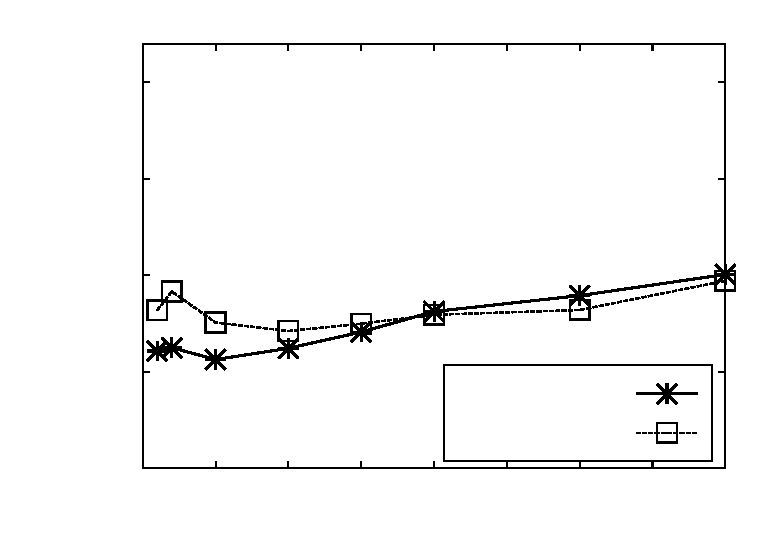
\includegraphics{graphs/database/a_read}}%
    \gplfronttext
  \end{picture}%
\endgroup
}} 
  \subfloat[][\textbf{Workload A:} update operations]{\resizebox{0.45\linewidth}{!}{% GNUPLOT: LaTeX picture with Postscript
\begingroup
  \makeatletter
  \providecommand\color[2][]{%
    \GenericError{(gnuplot) \space\space\space\@spaces}{%
      Package color not loaded in conjunction with
      terminal option `colourtext'%
    }{See the gnuplot documentation for explanation.%
    }{Either use 'blacktext' in gnuplot or load the package
      color.sty in LaTeX.}%
    \renewcommand\color[2][]{}%
  }%
  \providecommand\includegraphics[2][]{%
    \GenericError{(gnuplot) \space\space\space\@spaces}{%
      Package graphicx or graphics not loaded%
    }{See the gnuplot documentation for explanation.%
    }{The gnuplot epslatex terminal needs graphicx.sty or graphics.sty.}%
    \renewcommand\includegraphics[2][]{}%
  }%
  \providecommand\rotatebox[2]{#2}%
  \@ifundefined{ifGPcolor}{%
    \newif\ifGPcolor
    \GPcolorfalse
  }{}%
  \@ifundefined{ifGPblacktext}{%
    \newif\ifGPblacktext
    \GPblacktexttrue
  }{}%
  % define a \g@addto@macro without @ in the name:
  \let\gplgaddtomacro\g@addto@macro
  % define empty templates for all commands taking text:
  \gdef\gplbacktext{}%
  \gdef\gplfronttext{}%
  \makeatother
  \ifGPblacktext
    % no textcolor at all
    \def\colorrgb#1{}%
    \def\colorgray#1{}%
  \else
    % gray or color?
    \ifGPcolor
      \def\colorrgb#1{\color[rgb]{#1}}%
      \def\colorgray#1{\color[gray]{#1}}%
      \expandafter\def\csname LTw\endcsname{\color{white}}%
      \expandafter\def\csname LTb\endcsname{\color{black}}%
      \expandafter\def\csname LTa\endcsname{\color{black}}%
      \expandafter\def\csname LT0\endcsname{\color[rgb]{1,0,0}}%
      \expandafter\def\csname LT1\endcsname{\color[rgb]{0,1,0}}%
      \expandafter\def\csname LT2\endcsname{\color[rgb]{0,0,1}}%
      \expandafter\def\csname LT3\endcsname{\color[rgb]{1,0,1}}%
      \expandafter\def\csname LT4\endcsname{\color[rgb]{0,1,1}}%
      \expandafter\def\csname LT5\endcsname{\color[rgb]{1,1,0}}%
      \expandafter\def\csname LT6\endcsname{\color[rgb]{0,0,0}}%
      \expandafter\def\csname LT7\endcsname{\color[rgb]{1,0.3,0}}%
      \expandafter\def\csname LT8\endcsname{\color[rgb]{0.5,0.5,0.5}}%
    \else
      % gray
      \def\colorrgb#1{\color{black}}%
      \def\colorgray#1{\color[gray]{#1}}%
      \expandafter\def\csname LTw\endcsname{\color{white}}%
      \expandafter\def\csname LTb\endcsname{\color{black}}%
      \expandafter\def\csname LTa\endcsname{\color{black}}%
      \expandafter\def\csname LT0\endcsname{\color{black}}%
      \expandafter\def\csname LT1\endcsname{\color{black}}%
      \expandafter\def\csname LT2\endcsname{\color{black}}%
      \expandafter\def\csname LT3\endcsname{\color{black}}%
      \expandafter\def\csname LT4\endcsname{\color{black}}%
      \expandafter\def\csname LT5\endcsname{\color{black}}%
      \expandafter\def\csname LT6\endcsname{\color{black}}%
      \expandafter\def\csname LT7\endcsname{\color{black}}%
      \expandafter\def\csname LT8\endcsname{\color{black}}%
    \fi
  \fi
  \setlength{\unitlength}{0.0500bp}%
  \begin{picture}(7200.00,5040.00)%
    \gplgaddtomacro\gplbacktext{%
      \csname LTb\endcsname%
      \put(1078,704){\makebox(0,0)[r]{\strut{} 0}}%
      \put(1078,1629){\makebox(0,0)[r]{\strut{} 500}}%
      \put(1078,2554){\makebox(0,0)[r]{\strut{} 1000}}%
      \put(1078,3480){\makebox(0,0)[r]{\strut{} 1500}}%
      \put(1078,4405){\makebox(0,0)[r]{\strut{} 2000}}%
      \put(1210,484){\makebox(0,0){\strut{} 5}}%
      \put(2009,484){\makebox(0,0){\strut{} 10}}%
      \put(2808,484){\makebox(0,0){\strut{} 15}}%
      \put(3607,484){\makebox(0,0){\strut{} 20}}%
      \put(4406,484){\makebox(0,0){\strut{} 25}}%
      \put(5205,484){\makebox(0,0){\strut{} 30}}%
      \put(6004,484){\makebox(0,0){\strut{} 35}}%
      \put(6803,484){\makebox(0,0){\strut{} 40}}%
      \put(176,2739){\rotatebox{-270}{\makebox(0,0){\strut{}Update latency (us)}}}%
      \put(4006,154){\makebox(0,0){\strut{}Throughput (thousand ops/sec)}}%
    }%
    \gplgaddtomacro\gplfronttext{%
      \csname LTb\endcsname%
      \put(5816,1416){\makebox(0,0)[r]{\strut{}Shuttle}}%
      \csname LTb\endcsname%
      \put(5816,1042){\makebox(0,0)[r]{\strut{}No Shuttle}}%
    }%
    \gplbacktext
    \put(0,0){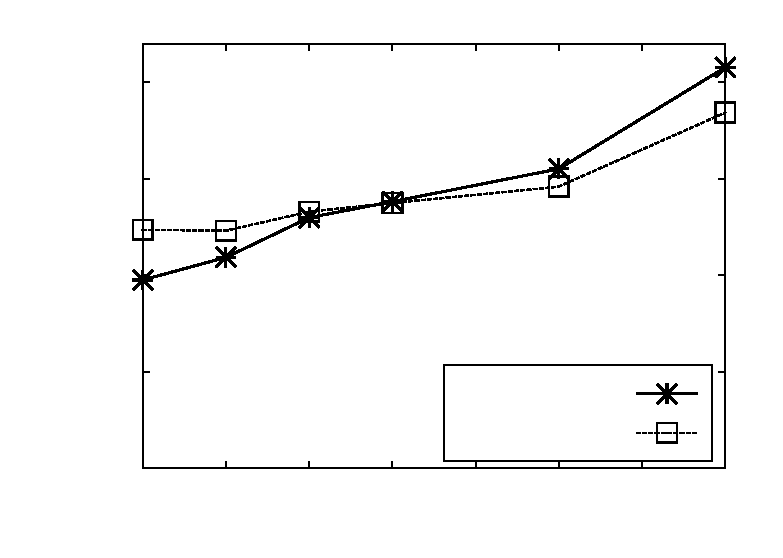
\includegraphics{graphs/database/a_update}}%
    \gplfronttext
  \end{picture}%
\endgroup
}}

  \subfloat[][\textbf{Workload B:} read operations]{\resizebox{0.45\linewidth}{!}{% GNUPLOT: LaTeX picture with Postscript
\begingroup
  \makeatletter
  \providecommand\color[2][]{%
    \GenericError{(gnuplot) \space\space\space\@spaces}{%
      Package color not loaded in conjunction with
      terminal option `colourtext'%
    }{See the gnuplot documentation for explanation.%
    }{Either use 'blacktext' in gnuplot or load the package
      color.sty in LaTeX.}%
    \renewcommand\color[2][]{}%
  }%
  \providecommand\includegraphics[2][]{%
    \GenericError{(gnuplot) \space\space\space\@spaces}{%
      Package graphicx or graphics not loaded%
    }{See the gnuplot documentation for explanation.%
    }{The gnuplot epslatex terminal needs graphicx.sty or graphics.sty.}%
    \renewcommand\includegraphics[2][]{}%
  }%
  \providecommand\rotatebox[2]{#2}%
  \@ifundefined{ifGPcolor}{%
    \newif\ifGPcolor
    \GPcolorfalse
  }{}%
  \@ifundefined{ifGPblacktext}{%
    \newif\ifGPblacktext
    \GPblacktexttrue
  }{}%
  % define a \g@addto@macro without @ in the name:
  \let\gplgaddtomacro\g@addto@macro
  % define empty templates for all commands taking text:
  \gdef\gplbacktext{}%
  \gdef\gplfronttext{}%
  \makeatother
  \ifGPblacktext
    % no textcolor at all
    \def\colorrgb#1{}%
    \def\colorgray#1{}%
  \else
    % gray or color?
    \ifGPcolor
      \def\colorrgb#1{\color[rgb]{#1}}%
      \def\colorgray#1{\color[gray]{#1}}%
      \expandafter\def\csname LTw\endcsname{\color{white}}%
      \expandafter\def\csname LTb\endcsname{\color{black}}%
      \expandafter\def\csname LTa\endcsname{\color{black}}%
      \expandafter\def\csname LT0\endcsname{\color[rgb]{1,0,0}}%
      \expandafter\def\csname LT1\endcsname{\color[rgb]{0,1,0}}%
      \expandafter\def\csname LT2\endcsname{\color[rgb]{0,0,1}}%
      \expandafter\def\csname LT3\endcsname{\color[rgb]{1,0,1}}%
      \expandafter\def\csname LT4\endcsname{\color[rgb]{0,1,1}}%
      \expandafter\def\csname LT5\endcsname{\color[rgb]{1,1,0}}%
      \expandafter\def\csname LT6\endcsname{\color[rgb]{0,0,0}}%
      \expandafter\def\csname LT7\endcsname{\color[rgb]{1,0.3,0}}%
      \expandafter\def\csname LT8\endcsname{\color[rgb]{0.5,0.5,0.5}}%
    \else
      % gray
      \def\colorrgb#1{\color{black}}%
      \def\colorgray#1{\color[gray]{#1}}%
      \expandafter\def\csname LTw\endcsname{\color{white}}%
      \expandafter\def\csname LTb\endcsname{\color{black}}%
      \expandafter\def\csname LTa\endcsname{\color{black}}%
      \expandafter\def\csname LT0\endcsname{\color{black}}%
      \expandafter\def\csname LT1\endcsname{\color{black}}%
      \expandafter\def\csname LT2\endcsname{\color{black}}%
      \expandafter\def\csname LT3\endcsname{\color{black}}%
      \expandafter\def\csname LT4\endcsname{\color{black}}%
      \expandafter\def\csname LT5\endcsname{\color{black}}%
      \expandafter\def\csname LT6\endcsname{\color{black}}%
      \expandafter\def\csname LT7\endcsname{\color{black}}%
      \expandafter\def\csname LT8\endcsname{\color{black}}%
    \fi
  \fi
  \setlength{\unitlength}{0.0500bp}%
  \begin{picture}(7200.00,5040.00)%
    \gplgaddtomacro\gplbacktext{%
      \csname LTb\endcsname%
      \put(1078,704){\makebox(0,0)[r]{\strut{} 0}}%
      \put(1078,1629){\makebox(0,0)[r]{\strut{} 500}}%
      \put(1078,2554){\makebox(0,0)[r]{\strut{} 1000}}%
      \put(1078,3480){\makebox(0,0)[r]{\strut{} 1500}}%
      \put(1078,4405){\makebox(0,0)[r]{\strut{} 2000}}%
      \put(1210,484){\makebox(0,0){\strut{} 5}}%
      \put(2009,484){\makebox(0,0){\strut{} 10}}%
      \put(2808,484){\makebox(0,0){\strut{} 15}}%
      \put(3607,484){\makebox(0,0){\strut{} 20}}%
      \put(4406,484){\makebox(0,0){\strut{} 25}}%
      \put(5205,484){\makebox(0,0){\strut{} 30}}%
      \put(6004,484){\makebox(0,0){\strut{} 35}}%
      \put(6803,484){\makebox(0,0){\strut{} 40}}%
      \put(176,2739){\rotatebox{-270}{\makebox(0,0){\strut{}Read latency (us)}}}%
      \put(4006,154){\makebox(0,0){\strut{}Throughput (thousand ops/sec)}}%
    }%
    \gplgaddtomacro\gplfronttext{%
      \csname LTb\endcsname%
      \put(5816,1416){\makebox(0,0)[r]{\strut{}Shuttle}}%
      \csname LTb\endcsname%
      \put(5816,1042){\makebox(0,0)[r]{\strut{}No Shuttle}}%
    }%
    \gplbacktext
    \put(0,0){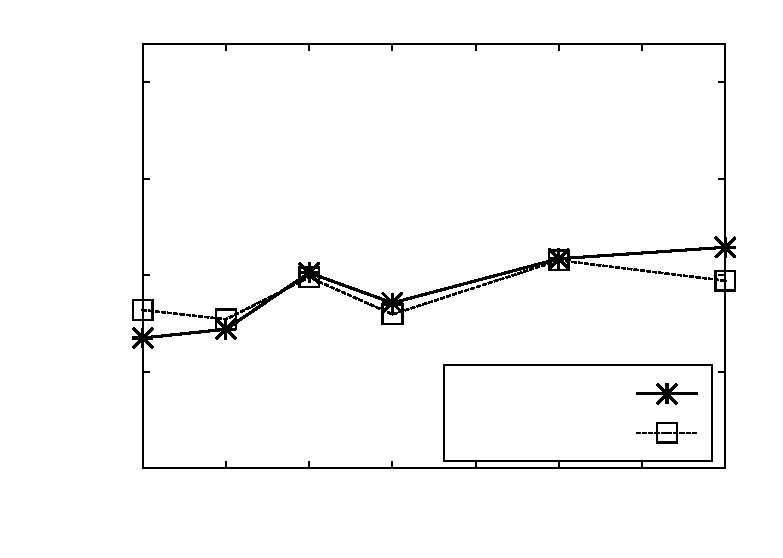
\includegraphics{graphs/database/b_read}}%
    \gplfronttext
  \end{picture}%
\endgroup
}} 
  \subfloat[][\textbf{Workload B:} update operations]{\resizebox{0.45\linewidth}{!}{% GNUPLOT: LaTeX picture with Postscript
\begingroup
  \makeatletter
  \providecommand\color[2][]{%
    \GenericError{(gnuplot) \space\space\space\@spaces}{%
      Package color not loaded in conjunction with
      terminal option `colourtext'%
    }{See the gnuplot documentation for explanation.%
    }{Either use 'blacktext' in gnuplot or load the package
      color.sty in LaTeX.}%
    \renewcommand\color[2][]{}%
  }%
  \providecommand\includegraphics[2][]{%
    \GenericError{(gnuplot) \space\space\space\@spaces}{%
      Package graphicx or graphics not loaded%
    }{See the gnuplot documentation for explanation.%
    }{The gnuplot epslatex terminal needs graphicx.sty or graphics.sty.}%
    \renewcommand\includegraphics[2][]{}%
  }%
  \providecommand\rotatebox[2]{#2}%
  \@ifundefined{ifGPcolor}{%
    \newif\ifGPcolor
    \GPcolorfalse
  }{}%
  \@ifundefined{ifGPblacktext}{%
    \newif\ifGPblacktext
    \GPblacktexttrue
  }{}%
  % define a \g@addto@macro without @ in the name:
  \let\gplgaddtomacro\g@addto@macro
  % define empty templates for all commands taking text:
  \gdef\gplbacktext{}%
  \gdef\gplfronttext{}%
  \makeatother
  \ifGPblacktext
    % no textcolor at all
    \def\colorrgb#1{}%
    \def\colorgray#1{}%
  \else
    % gray or color?
    \ifGPcolor
      \def\colorrgb#1{\color[rgb]{#1}}%
      \def\colorgray#1{\color[gray]{#1}}%
      \expandafter\def\csname LTw\endcsname{\color{white}}%
      \expandafter\def\csname LTb\endcsname{\color{black}}%
      \expandafter\def\csname LTa\endcsname{\color{black}}%
      \expandafter\def\csname LT0\endcsname{\color[rgb]{1,0,0}}%
      \expandafter\def\csname LT1\endcsname{\color[rgb]{0,1,0}}%
      \expandafter\def\csname LT2\endcsname{\color[rgb]{0,0,1}}%
      \expandafter\def\csname LT3\endcsname{\color[rgb]{1,0,1}}%
      \expandafter\def\csname LT4\endcsname{\color[rgb]{0,1,1}}%
      \expandafter\def\csname LT5\endcsname{\color[rgb]{1,1,0}}%
      \expandafter\def\csname LT6\endcsname{\color[rgb]{0,0,0}}%
      \expandafter\def\csname LT7\endcsname{\color[rgb]{1,0.3,0}}%
      \expandafter\def\csname LT8\endcsname{\color[rgb]{0.5,0.5,0.5}}%
    \else
      % gray
      \def\colorrgb#1{\color{black}}%
      \def\colorgray#1{\color[gray]{#1}}%
      \expandafter\def\csname LTw\endcsname{\color{white}}%
      \expandafter\def\csname LTb\endcsname{\color{black}}%
      \expandafter\def\csname LTa\endcsname{\color{black}}%
      \expandafter\def\csname LT0\endcsname{\color{black}}%
      \expandafter\def\csname LT1\endcsname{\color{black}}%
      \expandafter\def\csname LT2\endcsname{\color{black}}%
      \expandafter\def\csname LT3\endcsname{\color{black}}%
      \expandafter\def\csname LT4\endcsname{\color{black}}%
      \expandafter\def\csname LT5\endcsname{\color{black}}%
      \expandafter\def\csname LT6\endcsname{\color{black}}%
      \expandafter\def\csname LT7\endcsname{\color{black}}%
      \expandafter\def\csname LT8\endcsname{\color{black}}%
    \fi
  \fi
  \setlength{\unitlength}{0.0500bp}%
  \begin{picture}(7200.00,5040.00)%
    \gplgaddtomacro\gplbacktext{%
      \csname LTb\endcsname%
      \put(1078,704){\makebox(0,0)[r]{\strut{} 0}}%
      \put(1078,1629){\makebox(0,0)[r]{\strut{} 500}}%
      \put(1078,2554){\makebox(0,0)[r]{\strut{} 1000}}%
      \put(1078,3480){\makebox(0,0)[r]{\strut{} 1500}}%
      \put(1078,4405){\makebox(0,0)[r]{\strut{} 2000}}%
      \put(1210,484){\makebox(0,0){\strut{} 0}}%
      \put(1909,484){\makebox(0,0){\strut{} 5}}%
      \put(2608,484){\makebox(0,0){\strut{} 10}}%
      \put(3307,484){\makebox(0,0){\strut{} 15}}%
      \put(4007,484){\makebox(0,0){\strut{} 20}}%
      \put(4706,484){\makebox(0,0){\strut{} 25}}%
      \put(5405,484){\makebox(0,0){\strut{} 30}}%
      \put(6104,484){\makebox(0,0){\strut{} 35}}%
      \put(6803,484){\makebox(0,0){\strut{} 40}}%
      \put(176,2739){\rotatebox{-270}{\makebox(0,0){\strut{}Update latency (us)}}}%
      \put(4006,154){\makebox(0,0){\strut{}Throughput (thousand ops/sec)}}%
    }%
    \gplgaddtomacro\gplfronttext{%
      \csname LTb\endcsname%
      \put(5816,1416){\makebox(0,0)[r]{\strut{}Shuttle}}%
      \csname LTb\endcsname%
      \put(5816,1042){\makebox(0,0)[r]{\strut{}No Shuttle}}%
    }%
    \gplbacktext
    \put(0,0){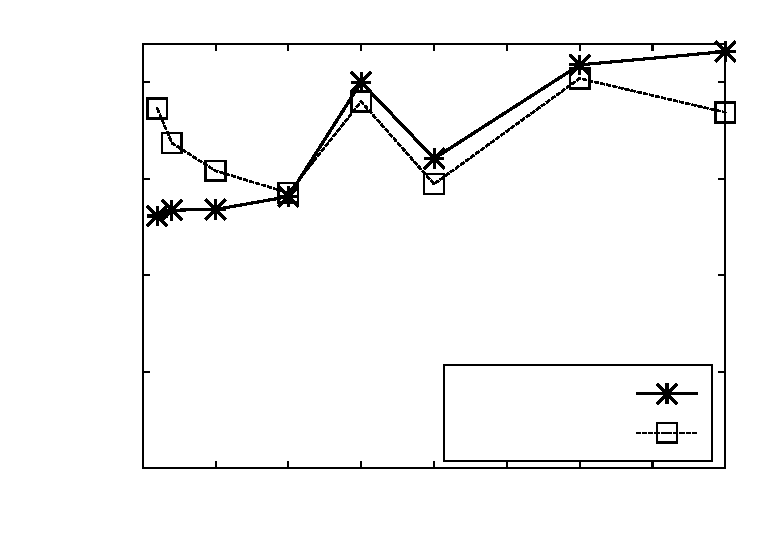
\includegraphics{graphs/database/b_update}}%
    \gplfronttext
  \end{picture}%
\endgroup
}}

  \subfloat[][\textbf{Workload C:} read operations]{\resizebox{0.45\linewidth}{!}{% GNUPLOT: LaTeX picture with Postscript
\begingroup
  \makeatletter
  \providecommand\color[2][]{%
    \GenericError{(gnuplot) \space\space\space\@spaces}{%
      Package color not loaded in conjunction with
      terminal option `colourtext'%
    }{See the gnuplot documentation for explanation.%
    }{Either use 'blacktext' in gnuplot or load the package
      color.sty in LaTeX.}%
    \renewcommand\color[2][]{}%
  }%
  \providecommand\includegraphics[2][]{%
    \GenericError{(gnuplot) \space\space\space\@spaces}{%
      Package graphicx or graphics not loaded%
    }{See the gnuplot documentation for explanation.%
    }{The gnuplot epslatex terminal needs graphicx.sty or graphics.sty.}%
    \renewcommand\includegraphics[2][]{}%
  }%
  \providecommand\rotatebox[2]{#2}%
  \@ifundefined{ifGPcolor}{%
    \newif\ifGPcolor
    \GPcolorfalse
  }{}%
  \@ifundefined{ifGPblacktext}{%
    \newif\ifGPblacktext
    \GPblacktexttrue
  }{}%
  % define a \g@addto@macro without @ in the name:
  \let\gplgaddtomacro\g@addto@macro
  % define empty templates for all commands taking text:
  \gdef\gplbacktext{}%
  \gdef\gplfronttext{}%
  \makeatother
  \ifGPblacktext
    % no textcolor at all
    \def\colorrgb#1{}%
    \def\colorgray#1{}%
  \else
    % gray or color?
    \ifGPcolor
      \def\colorrgb#1{\color[rgb]{#1}}%
      \def\colorgray#1{\color[gray]{#1}}%
      \expandafter\def\csname LTw\endcsname{\color{white}}%
      \expandafter\def\csname LTb\endcsname{\color{black}}%
      \expandafter\def\csname LTa\endcsname{\color{black}}%
      \expandafter\def\csname LT0\endcsname{\color[rgb]{1,0,0}}%
      \expandafter\def\csname LT1\endcsname{\color[rgb]{0,1,0}}%
      \expandafter\def\csname LT2\endcsname{\color[rgb]{0,0,1}}%
      \expandafter\def\csname LT3\endcsname{\color[rgb]{1,0,1}}%
      \expandafter\def\csname LT4\endcsname{\color[rgb]{0,1,1}}%
      \expandafter\def\csname LT5\endcsname{\color[rgb]{1,1,0}}%
      \expandafter\def\csname LT6\endcsname{\color[rgb]{0,0,0}}%
      \expandafter\def\csname LT7\endcsname{\color[rgb]{1,0.3,0}}%
      \expandafter\def\csname LT8\endcsname{\color[rgb]{0.5,0.5,0.5}}%
    \else
      % gray
      \def\colorrgb#1{\color{black}}%
      \def\colorgray#1{\color[gray]{#1}}%
      \expandafter\def\csname LTw\endcsname{\color{white}}%
      \expandafter\def\csname LTb\endcsname{\color{black}}%
      \expandafter\def\csname LTa\endcsname{\color{black}}%
      \expandafter\def\csname LT0\endcsname{\color{black}}%
      \expandafter\def\csname LT1\endcsname{\color{black}}%
      \expandafter\def\csname LT2\endcsname{\color{black}}%
      \expandafter\def\csname LT3\endcsname{\color{black}}%
      \expandafter\def\csname LT4\endcsname{\color{black}}%
      \expandafter\def\csname LT5\endcsname{\color{black}}%
      \expandafter\def\csname LT6\endcsname{\color{black}}%
      \expandafter\def\csname LT7\endcsname{\color{black}}%
      \expandafter\def\csname LT8\endcsname{\color{black}}%
    \fi
  \fi
  \setlength{\unitlength}{0.0500bp}%
  \begin{picture}(7200.00,5040.00)%
    \gplgaddtomacro\gplbacktext{%
      \csname LTb\endcsname%
      \put(1078,704){\makebox(0,0)[r]{\strut{} 0}}%
      \put(1078,1629){\makebox(0,0)[r]{\strut{} 500}}%
      \put(1078,2554){\makebox(0,0)[r]{\strut{} 1000}}%
      \put(1078,3480){\makebox(0,0)[r]{\strut{} 1500}}%
      \put(1078,4405){\makebox(0,0)[r]{\strut{} 2000}}%
      \put(1210,484){\makebox(0,0){\strut{} 0}}%
      \put(2142,484){\makebox(0,0){\strut{} 10}}%
      \put(3074,484){\makebox(0,0){\strut{} 20}}%
      \put(4007,484){\makebox(0,0){\strut{} 30}}%
      \put(4939,484){\makebox(0,0){\strut{} 40}}%
      \put(5871,484){\makebox(0,0){\strut{} 50}}%
      \put(6803,484){\makebox(0,0){\strut{} 60}}%
      \put(176,2739){\rotatebox{-270}{\makebox(0,0){\strut{}Read latency (us)}}}%
      \put(4006,154){\makebox(0,0){\strut{}Throughput (thousand ops/sec)}}%
    }%
    \gplgaddtomacro\gplfronttext{%
      \csname LTb\endcsname%
      \put(5816,1416){\makebox(0,0)[r]{\strut{}Shuttle}}%
      \csname LTb\endcsname%
      \put(5816,1042){\makebox(0,0)[r]{\strut{}No Shuttle}}%
    }%
    \gplbacktext
    \put(0,0){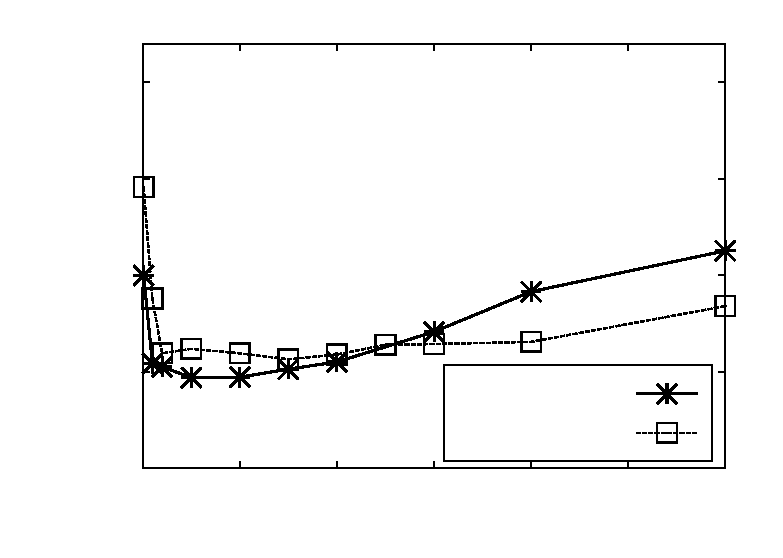
\includegraphics{graphs/database/c_read}}%
    \gplfronttext
  \end{picture}%
\endgroup
}} 

  \subfloat[][\textbf{Workload D:} read operations]{\resizebox{0.45\linewidth}{!}{% GNUPLOT: LaTeX picture with Postscript
\begingroup
  \makeatletter
  \providecommand\color[2][]{%
    \GenericError{(gnuplot) \space\space\space\@spaces}{%
      Package color not loaded in conjunction with
      terminal option `colourtext'%
    }{See the gnuplot documentation for explanation.%
    }{Either use 'blacktext' in gnuplot or load the package
      color.sty in LaTeX.}%
    \renewcommand\color[2][]{}%
  }%
  \providecommand\includegraphics[2][]{%
    \GenericError{(gnuplot) \space\space\space\@spaces}{%
      Package graphicx or graphics not loaded%
    }{See the gnuplot documentation for explanation.%
    }{The gnuplot epslatex terminal needs graphicx.sty or graphics.sty.}%
    \renewcommand\includegraphics[2][]{}%
  }%
  \providecommand\rotatebox[2]{#2}%
  \@ifundefined{ifGPcolor}{%
    \newif\ifGPcolor
    \GPcolorfalse
  }{}%
  \@ifundefined{ifGPblacktext}{%
    \newif\ifGPblacktext
    \GPblacktexttrue
  }{}%
  % define a \g@addto@macro without @ in the name:
  \let\gplgaddtomacro\g@addto@macro
  % define empty templates for all commands taking text:
  \gdef\gplbacktext{}%
  \gdef\gplfronttext{}%
  \makeatother
  \ifGPblacktext
    % no textcolor at all
    \def\colorrgb#1{}%
    \def\colorgray#1{}%
  \else
    % gray or color?
    \ifGPcolor
      \def\colorrgb#1{\color[rgb]{#1}}%
      \def\colorgray#1{\color[gray]{#1}}%
      \expandafter\def\csname LTw\endcsname{\color{white}}%
      \expandafter\def\csname LTb\endcsname{\color{black}}%
      \expandafter\def\csname LTa\endcsname{\color{black}}%
      \expandafter\def\csname LT0\endcsname{\color[rgb]{1,0,0}}%
      \expandafter\def\csname LT1\endcsname{\color[rgb]{0,1,0}}%
      \expandafter\def\csname LT2\endcsname{\color[rgb]{0,0,1}}%
      \expandafter\def\csname LT3\endcsname{\color[rgb]{1,0,1}}%
      \expandafter\def\csname LT4\endcsname{\color[rgb]{0,1,1}}%
      \expandafter\def\csname LT5\endcsname{\color[rgb]{1,1,0}}%
      \expandafter\def\csname LT6\endcsname{\color[rgb]{0,0,0}}%
      \expandafter\def\csname LT7\endcsname{\color[rgb]{1,0.3,0}}%
      \expandafter\def\csname LT8\endcsname{\color[rgb]{0.5,0.5,0.5}}%
    \else
      % gray
      \def\colorrgb#1{\color{black}}%
      \def\colorgray#1{\color[gray]{#1}}%
      \expandafter\def\csname LTw\endcsname{\color{white}}%
      \expandafter\def\csname LTb\endcsname{\color{black}}%
      \expandafter\def\csname LTa\endcsname{\color{black}}%
      \expandafter\def\csname LT0\endcsname{\color{black}}%
      \expandafter\def\csname LT1\endcsname{\color{black}}%
      \expandafter\def\csname LT2\endcsname{\color{black}}%
      \expandafter\def\csname LT3\endcsname{\color{black}}%
      \expandafter\def\csname LT4\endcsname{\color{black}}%
      \expandafter\def\csname LT5\endcsname{\color{black}}%
      \expandafter\def\csname LT6\endcsname{\color{black}}%
      \expandafter\def\csname LT7\endcsname{\color{black}}%
      \expandafter\def\csname LT8\endcsname{\color{black}}%
    \fi
  \fi
  \setlength{\unitlength}{0.0500bp}%
  \begin{picture}(7200.00,5040.00)%
    \gplgaddtomacro\gplbacktext{%
      \csname LTb\endcsname%
      \put(1078,704){\makebox(0,0)[r]{\strut{} 0}}%
      \put(1078,1629){\makebox(0,0)[r]{\strut{} 500}}%
      \put(1078,2554){\makebox(0,0)[r]{\strut{} 1000}}%
      \put(1078,3480){\makebox(0,0)[r]{\strut{} 1500}}%
      \put(1078,4405){\makebox(0,0)[r]{\strut{} 2000}}%
      \put(1210,484){\makebox(0,0){\strut{} 0}}%
      \put(1909,484){\makebox(0,0){\strut{} 5}}%
      \put(2608,484){\makebox(0,0){\strut{} 10}}%
      \put(3307,484){\makebox(0,0){\strut{} 15}}%
      \put(4007,484){\makebox(0,0){\strut{} 20}}%
      \put(4706,484){\makebox(0,0){\strut{} 25}}%
      \put(5405,484){\makebox(0,0){\strut{} 30}}%
      \put(6104,484){\makebox(0,0){\strut{} 35}}%
      \put(6803,484){\makebox(0,0){\strut{} 40}}%
      \put(176,2739){\rotatebox{-270}{\makebox(0,0){\strut{}Read latency (us)}}}%
      \put(4006,154){\makebox(0,0){\strut{}Throughput (thousand ops/sec)}}%
    }%
    \gplgaddtomacro\gplfronttext{%
      \csname LTb\endcsname%
      \put(5816,1416){\makebox(0,0)[r]{\strut{}Shuttle}}%
      \csname LTb\endcsname%
      \put(5816,1042){\makebox(0,0)[r]{\strut{}No Shuttle}}%
    }%
    \gplbacktext
    \put(0,0){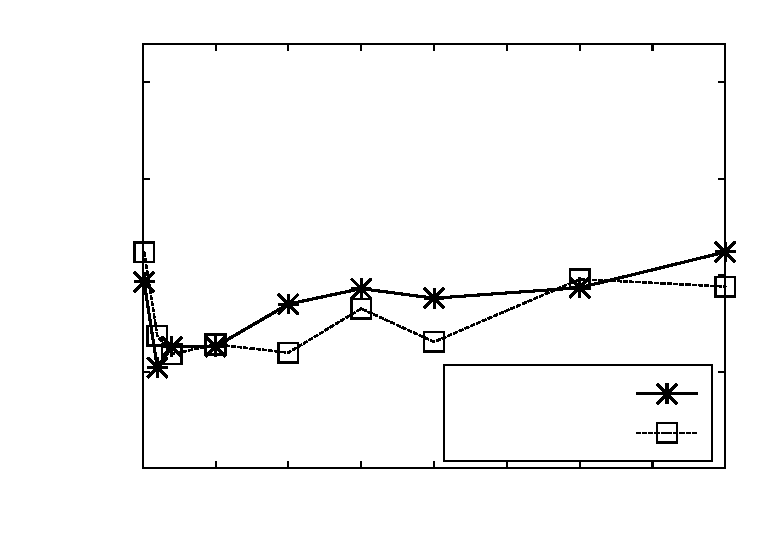
\includegraphics{graphs/database/d_read}}%
    \gplfronttext
  \end{picture}%
\endgroup
}} 
  \subfloat[][\textbf{Workload D:} insert operations]{\resizebox{0.45\linewidth}{!}{% GNUPLOT: LaTeX picture with Postscript
\begingroup
  \makeatletter
  \providecommand\color[2][]{%
    \GenericError{(gnuplot) \space\space\space\@spaces}{%
      Package color not loaded in conjunction with
      terminal option `colourtext'%
    }{See the gnuplot documentation for explanation.%
    }{Either use 'blacktext' in gnuplot or load the package
      color.sty in LaTeX.}%
    \renewcommand\color[2][]{}%
  }%
  \providecommand\includegraphics[2][]{%
    \GenericError{(gnuplot) \space\space\space\@spaces}{%
      Package graphicx or graphics not loaded%
    }{See the gnuplot documentation for explanation.%
    }{The gnuplot epslatex terminal needs graphicx.sty or graphics.sty.}%
    \renewcommand\includegraphics[2][]{}%
  }%
  \providecommand\rotatebox[2]{#2}%
  \@ifundefined{ifGPcolor}{%
    \newif\ifGPcolor
    \GPcolorfalse
  }{}%
  \@ifundefined{ifGPblacktext}{%
    \newif\ifGPblacktext
    \GPblacktexttrue
  }{}%
  % define a \g@addto@macro without @ in the name:
  \let\gplgaddtomacro\g@addto@macro
  % define empty templates for all commands taking text:
  \gdef\gplbacktext{}%
  \gdef\gplfronttext{}%
  \makeatother
  \ifGPblacktext
    % no textcolor at all
    \def\colorrgb#1{}%
    \def\colorgray#1{}%
  \else
    % gray or color?
    \ifGPcolor
      \def\colorrgb#1{\color[rgb]{#1}}%
      \def\colorgray#1{\color[gray]{#1}}%
      \expandafter\def\csname LTw\endcsname{\color{white}}%
      \expandafter\def\csname LTb\endcsname{\color{black}}%
      \expandafter\def\csname LTa\endcsname{\color{black}}%
      \expandafter\def\csname LT0\endcsname{\color[rgb]{1,0,0}}%
      \expandafter\def\csname LT1\endcsname{\color[rgb]{0,1,0}}%
      \expandafter\def\csname LT2\endcsname{\color[rgb]{0,0,1}}%
      \expandafter\def\csname LT3\endcsname{\color[rgb]{1,0,1}}%
      \expandafter\def\csname LT4\endcsname{\color[rgb]{0,1,1}}%
      \expandafter\def\csname LT5\endcsname{\color[rgb]{1,1,0}}%
      \expandafter\def\csname LT6\endcsname{\color[rgb]{0,0,0}}%
      \expandafter\def\csname LT7\endcsname{\color[rgb]{1,0.3,0}}%
      \expandafter\def\csname LT8\endcsname{\color[rgb]{0.5,0.5,0.5}}%
    \else
      % gray
      \def\colorrgb#1{\color{black}}%
      \def\colorgray#1{\color[gray]{#1}}%
      \expandafter\def\csname LTw\endcsname{\color{white}}%
      \expandafter\def\csname LTb\endcsname{\color{black}}%
      \expandafter\def\csname LTa\endcsname{\color{black}}%
      \expandafter\def\csname LT0\endcsname{\color{black}}%
      \expandafter\def\csname LT1\endcsname{\color{black}}%
      \expandafter\def\csname LT2\endcsname{\color{black}}%
      \expandafter\def\csname LT3\endcsname{\color{black}}%
      \expandafter\def\csname LT4\endcsname{\color{black}}%
      \expandafter\def\csname LT5\endcsname{\color{black}}%
      \expandafter\def\csname LT6\endcsname{\color{black}}%
      \expandafter\def\csname LT7\endcsname{\color{black}}%
      \expandafter\def\csname LT8\endcsname{\color{black}}%
    \fi
  \fi
  \setlength{\unitlength}{0.0500bp}%
  \begin{picture}(7200.00,5040.00)%
    \gplgaddtomacro\gplbacktext{%
      \csname LTb\endcsname%
      \put(1078,704){\makebox(0,0)[r]{\strut{} 0}}%
      \put(1078,1629){\makebox(0,0)[r]{\strut{} 500}}%
      \put(1078,2554){\makebox(0,0)[r]{\strut{} 1000}}%
      \put(1078,3480){\makebox(0,0)[r]{\strut{} 1500}}%
      \put(1078,4405){\makebox(0,0)[r]{\strut{} 2000}}%
      \put(1210,484){\makebox(0,0){\strut{} 0}}%
      \put(1909,484){\makebox(0,0){\strut{} 5}}%
      \put(2608,484){\makebox(0,0){\strut{} 10}}%
      \put(3307,484){\makebox(0,0){\strut{} 15}}%
      \put(4007,484){\makebox(0,0){\strut{} 20}}%
      \put(4706,484){\makebox(0,0){\strut{} 25}}%
      \put(5405,484){\makebox(0,0){\strut{} 30}}%
      \put(6104,484){\makebox(0,0){\strut{} 35}}%
      \put(6803,484){\makebox(0,0){\strut{} 40}}%
      \put(176,2739){\rotatebox{-270}{\makebox(0,0){\strut{}Insert latency (us)}}}%
      \put(4006,154){\makebox(0,0){\strut{}Throughput (thousand ops/sec)}}%
    }%
    \gplgaddtomacro\gplfronttext{%
      \csname LTb\endcsname%
      \put(5816,1416){\makebox(0,0)[r]{\strut{}Shuttle}}%
      \csname LTb\endcsname%
      \put(5816,1042){\makebox(0,0)[r]{\strut{}No Shuttle}}%
    }%
    \gplbacktext
    \put(0,0){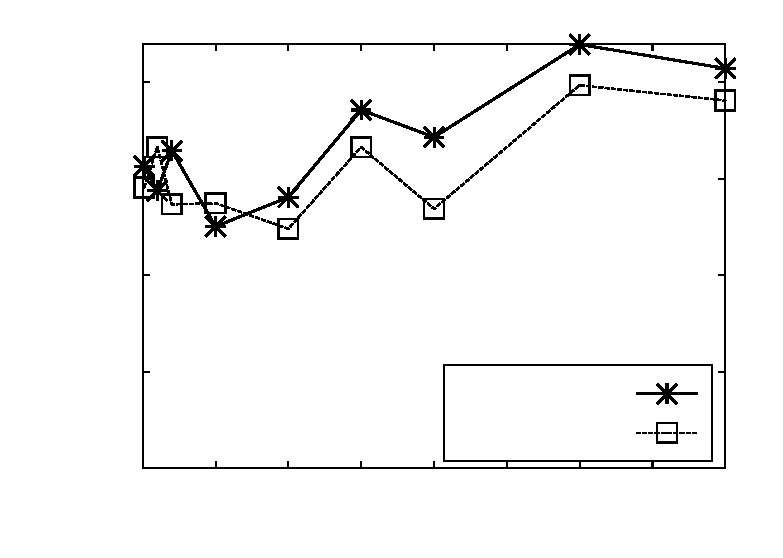
\includegraphics{graphs/database/d_insert}}%
    \gplfronttext
  \end{picture}%
\endgroup
}}
  \caption{Shuttle overhead on database}
  \label{fig:database_overhead_workloads}
\end{figure}

We expected the major Shuttle impact on database to be the read-write lock. Shuttle serializes the requests per-key using a read-write lock. In addition, the underlying \acf{BDB}, which is used by Voldemort as persistent-storage, also uses a read-write lock. However, the results in Figure \ref{fig:database_overhead_workloads} prove that Shuttle imposes a negligible latency overhead for the various types of workload and request rate.  

Shuttle also iterates over the \emph{operation lists} to determine the dependencies and sends them to the \emph{manager}. The instance's CPU usage was 10\% in average and the throughput did not reveal any variation when the dependencies are being collected. 

Shuttle snapshot mechanism requires creating a new data item in the Voldemort database and creating a new data version. A new version takes 264.077\us (standard deviation 864.293\us) to be created, while overwrite a version takes 266.635\us (std. deviation 577.124\us).

We conclude that Shuttle database proxy does not represent a significant performance overhead. %medi 1 milhao de entradas no meu computador


%---------------------------------- proxy ----------------------------------
\subsubsection{Proxy}\label{sec:eval:performance:proxy}
We setup an environment with 3 \ac{AWS} \textit{c3.xlarge} instances to measure the proxy overhead. The first runs a \ac{HTTP} benchmark tool \emph{weighttp} \cite{weighttp}. The second runs a HAProxy (v1.5.3) as load balancer and the Shuttle's proxy. The third runs a WildFly serving a 1KB static file. The benchmark tool performed 2 million requests using 8 threads and 200 clients.

\begin{figure}
  \begin{minipage}[t][][b]{0.55\linewidth}
    \resizebox{8cm}{!} {% GNUPLOT: LaTeX picture with Postscript
\begingroup
  \makeatletter
  \providecommand\color[2][]{%
    \GenericError{(gnuplot) \space\space\space\@spaces}{%
      Package color not loaded in conjunction with
      terminal option `colourtext'%
    }{See the gnuplot documentation for explanation.%
    }{Either use 'blacktext' in gnuplot or load the package
      color.sty in LaTeX.}%
    \renewcommand\color[2][]{}%
  }%
  \providecommand\includegraphics[2][]{%
    \GenericError{(gnuplot) \space\space\space\@spaces}{%
      Package graphicx or graphics not loaded%
    }{See the gnuplot documentation for explanation.%
    }{The gnuplot epslatex terminal needs graphicx.sty or graphics.sty.}%
    \renewcommand\includegraphics[2][]{}%
  }%
  \providecommand\rotatebox[2]{#2}%
  \@ifundefined{ifGPcolor}{%
    \newif\ifGPcolor
    \GPcolorfalse
  }{}%
  \@ifundefined{ifGPblacktext}{%
    \newif\ifGPblacktext
    \GPblacktexttrue
  }{}%
  % define a \g@addto@macro without @ in the name:
  \let\gplgaddtomacro\g@addto@macro
  % define empty templates for all commands taking text:
  \gdef\gplbacktext{}%
  \gdef\gplfronttext{}%
  \makeatother
  \ifGPblacktext
    % no textcolor at all
    \def\colorrgb#1{}%
    \def\colorgray#1{}%
  \else
    % gray or color?
    \ifGPcolor
      \def\colorrgb#1{\color[rgb]{#1}}%
      \def\colorgray#1{\color[gray]{#1}}%
      \expandafter\def\csname LTw\endcsname{\color{white}}%
      \expandafter\def\csname LTb\endcsname{\color{black}}%
      \expandafter\def\csname LTa\endcsname{\color{black}}%
      \expandafter\def\csname LT0\endcsname{\color[rgb]{1,0,0}}%
      \expandafter\def\csname LT1\endcsname{\color[rgb]{0,1,0}}%
      \expandafter\def\csname LT2\endcsname{\color[rgb]{0,0,1}}%
      \expandafter\def\csname LT3\endcsname{\color[rgb]{1,0,1}}%
      \expandafter\def\csname LT4\endcsname{\color[rgb]{0,1,1}}%
      \expandafter\def\csname LT5\endcsname{\color[rgb]{1,1,0}}%
      \expandafter\def\csname LT6\endcsname{\color[rgb]{0,0,0}}%
      \expandafter\def\csname LT7\endcsname{\color[rgb]{1,0.3,0}}%
      \expandafter\def\csname LT8\endcsname{\color[rgb]{0.5,0.5,0.5}}%
    \else
      % gray
      \def\colorrgb#1{\color{black}}%
      \def\colorgray#1{\color[gray]{#1}}%
      \expandafter\def\csname LTw\endcsname{\color{white}}%
      \expandafter\def\csname LTb\endcsname{\color{black}}%
      \expandafter\def\csname LTa\endcsname{\color{black}}%
      \expandafter\def\csname LT0\endcsname{\color{black}}%
      \expandafter\def\csname LT1\endcsname{\color{black}}%
      \expandafter\def\csname LT2\endcsname{\color{black}}%
      \expandafter\def\csname LT3\endcsname{\color{black}}%
      \expandafter\def\csname LT4\endcsname{\color{black}}%
      \expandafter\def\csname LT5\endcsname{\color{black}}%
      \expandafter\def\csname LT6\endcsname{\color{black}}%
      \expandafter\def\csname LT7\endcsname{\color{black}}%
      \expandafter\def\csname LT8\endcsname{\color{black}}%
    \fi
  \fi
  \setlength{\unitlength}{0.0500bp}%
  \begin{picture}(7200.00,5040.00)%
    \gplgaddtomacro\gplbacktext{%
      \csname LTb\endcsname%
      \put(1210,440){\makebox(0,0)[r]{\strut{} 0}}%
      \put(1210,1018){\makebox(0,0)[r]{\strut{} 10000}}%
      \put(1210,1596){\makebox(0,0)[r]{\strut{} 20000}}%
      \put(1210,2174){\makebox(0,0)[r]{\strut{} 30000}}%
      \put(1210,2752){\makebox(0,0)[r]{\strut{} 40000}}%
      \put(1210,3330){\makebox(0,0)[r]{\strut{} 50000}}%
      \put(1210,3908){\makebox(0,0)[r]{\strut{} 60000}}%
      \put(1210,4486){\makebox(0,0)[r]{\strut{} 70000}}%
      \put(1645,220){\makebox(0,0){\strut{}a}}%
      \put(2859,220){\makebox(0,0){\strut{}b}}%
      \put(4073,220){\makebox(0,0){\strut{}c}}%
      \put(5286,220){\makebox(0,0){\strut{}d}}%
      \put(6500,220){\makebox(0,0){\strut{}e}}%
      \put(176,2607){\rotatebox{-270}{\makebox(0,0){\strut{}Requests per second}}}%
    }%
    \gplgaddtomacro\gplfronttext{%
    }%
    \gplbacktext
    \put(0,0){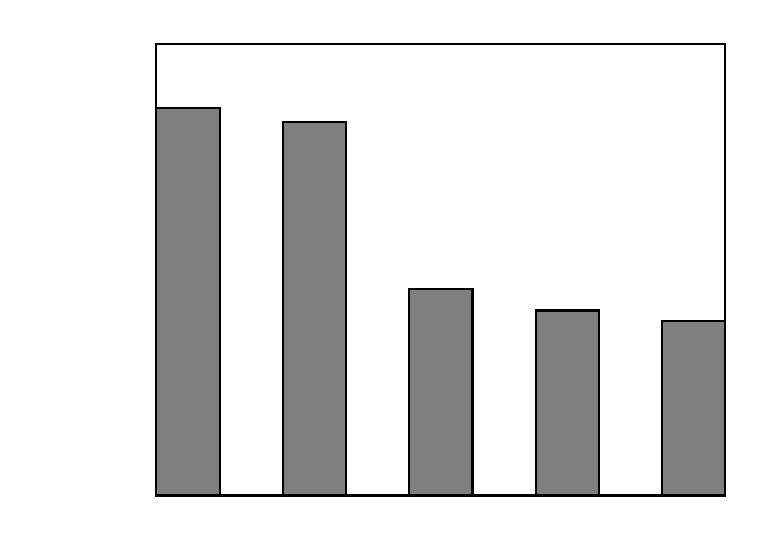
\includegraphics{graphs/proxy/throughput}}%
    \gplfronttext
  \end{picture}%
\endgroup
}
  \end{minipage}%
  \begin{minipage}[t][][b]{0.30\linewidth}
      \begin{tabular}{l|l|l|r}
            & \bf{Load Balancer} & \bf{Proxy}  & \bf{Latency (ms)}    \\ \hline
          a &                    &             & 1.08 (1.17)          \\
          b & \cmark             &             & 1.08 (1.25)          \\
          c &                    & \cmark      & 1.11 (1.28)          \\
          d & \cmark             & No log      & 1.10 (1.27)          \\
          e & \cmark             & \cmark      & 1.11 (1.29)          
      \end{tabular}
  \end{minipage}
\caption[Proxy Overhead]{Proxy Overhead: From left to right: direct to the server; only with the load balancer (HAProxy); Shuttle logging but without load balancer; overhead of Shuttle with load balancer when not logging and logging. The table describes the scenarios of the graph and the request latency (average and 95th percentile) in them. \hl{por favor, verifique a legenda. A tabela basicamente descreve o que o grafico tem e dá as latencias. É um bacoado manhoso}}
\label{fig:overhead_proxy}
\end{figure}

Figure \ref{fig:overhead_proxy} represents the throughput limit imposed by Shuttle's proxy. Shuttle's proxy imposes a considerable performance limitation (c) comparing with the load balancer (b). However, the logging mechanism has a negligible influence on the maximum request throughput (column \emph{d} comparing with column \emph{e}). In addition, the table in Figure \ref{fig:overhead_proxy} shows that Shuttle imposes a negligible overhead on requests latency considering a constant request income rate of 2500 requests per second. \hl{este parágrafo está bem escrito?}

We conclude that the performance overhead due to logging is negligible but the proxy is a considerable throughput limitation. The main cause is its implementation: while HAProxy is implemented using C and it is heavily optimized, Shuttle's proxy is a prototype implemented in Java. Therefore, we expect a C implementation of proxy can overcome the performance overhead. However, we claim that our prototype implementation is enough for most of small and enterprise services deployed in \ac{PaaS} because the throughput limit imposed by the proxy is lower than the request rates presented in Table \ref{tab:base_throughputs}. Moreover, the recovery time is dependent from the application performance but independent from the proxy's performance. \\  

%---------------------------------- webserver ----------------------------------
The overhead of Shuttle on each application server is database client interceptor that logs the accessed keys per request. Our experiments demonstrated that logging and storing the accessed keys implies a negligible overhead on the response latency.  \hl{este parágrafo fica um pouco deslocado certo? é só para não ter ficado nada por avaliar}


%---------------------------------- total ----------------------------------
\subsubsection{Total}\label{sec:eval:performance:total}
\hl{pois, total é uma marca de produtos petroquimicos. Eu não consegui arranjar um nome. Até aqui temos estado a ver parte a parte qual o overhead, aqui é do sistema completo, com tudo a funcionar}
We evaluate the overhead of Shuttle by measuring the throughput of the \textit{Ask} application with and without Shuttle (Table \ref{tab:throughput}). We do not consider a particular scenario or replay scheme (full/selective) but define instead the number of requests recovered per experiment. We run 6 \ac{AWS} \textit{c3.xlarge} instances. We use one client, one instance with Shuttle proxy and a load balancer (HAProxy), three WildFly application servers and one Voldemort database.

We considered two workloads: (A) has 50\% reads, 50\% inserts and (B) has 95\% reads, 5\% inserts. Insert operations adds questions, answers, comments and votes of the data sample, while read operations access the latest inserted questions. The insert operations insert the questions, answers, comments and votes of the data sample, while the read operations access the latest inserted questions. We consider a large data sample from \textit{StackExchange Data Dump} \cite{stackexchange_data} with 3 million requests (250812 questions, 335312 answers, 717937 comments, 1695939 votes).

Table \ref{tab:throughput} shows that Shuttle imposes an overhead of 13-20\%, which seems reasonable considering the benefits of having it. We believe the main cause of overhead is the current proxy, which is not very optimized. The current version written in Java performs considerably better than a previous version in Python, but we expect to be able to do much better by rewriting it in C. Still, while the proxy and database instances consume a low level of resources, the application instances consumed the maximum of CPU resources available.


\begin{table}
\centering
\begin{tabular}{l|rr}
                           &  \textbf{Workload A}   & \textbf{Workload B}  \\ \hline
\textbf{Shuttle}           &  6325 ops/sec [5.78 ms]  &  15346 ops/sec[3.62 ms]  \\
\textbf{No Shuttle}        &  7148 ops/sec [5.07 ms]  &  17821 ops/sec[3.01 ms]  \\
\end{tabular}
\caption{Shuttle overhead in terms of application throughput (ops/sec) and response latency (ms)}
\label{tab:throughput}
\end{table}

Considering the request rates presented in Table \ref{tab:base_throughputs}, we claim that a small environment with 6 machines is enough to support a small to medium application running with Shuttle. 

In conclusion, we prove that a single proxy architecture, which simplifies the Shuttle design by globally order the requests, is adequate. 




%%%%%%%%%%%%%%%%%%%%%%%%%%%%%%%%%%%%%%%%%%%%%%%%%%%%%%%%%%%%%%%%%%%%%%%%%%%%%%%%%%%%%%%%%%%%%%%%%%%%%%%%%%%%%%%%%%%%%%%%%%%%%%%%%%%%%%%


\subsection{Recovery}\label{sec:eval:recovery}
We measured the performance of the recovery process. We do not consider a particular scenario or replay scheme (full/selective) but define instead the number of requests recovered per experiment.

The recovery process can be summarized in the following points:

\begin{itemize}
  \item Generate the list of requests to replay;
  \item Launch replay instances; Launch new application servers and database instances, if instance rejuvenation is used;
  \item Replay the requests.
\end{itemize}

The main factors of influence on recovery performance are: 1) the number of requests to replay, which depends on the request arrival rate; 2) the detection delay; 3) the number and type of database operations of each request.


We setup a test environment with 6 \emph{c3.xlarge} instances in an \ac{AWS} \acf{VPC}, sharing the same placement group (Figure \ref{fig:aws_diagram}). The first instance runs the \emph{TryOut} testing application. The second runs Shuttle's manager, replay and Shuttle Storage (Cassandra). The third contains the application server WildFly with the application \emph{Ask}. The last instance runs the database.

\begin{figure}[!htb]
  \centering
  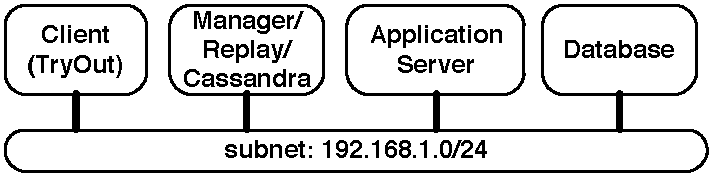
\includegraphics[width=90mm]{images/aws_diagram}
  \caption{Instances deployed on \ac{AWS} }
  \label{fig:aws_diagram}
\end{figure}


We considered a workload of 95\% reads, 5\% inserts (StackExchange network has a read/write ratio of 98.82\%). We consider a subset of \textit{StackExchange Data Dump} \cite{stackexchange_data} with 50 000 insert request (1432 questions, 3399 answers, 8335 comments, 36834 votes). Therefore, we consider a total of 1 million requests. The selected questions had 899 407 views in StackExchange. We consider 950 000 view requests. 

TryOut performed the 1 million requests in 672 seconds on average (1486 requests/second, standard deviation of 20 seconds) using 25 concurrent threads (Figure \ref{fig:recovery_period}). The average response latency was 15.82\ms (90th percentile of 22.826\ms and 95th of 27.721\ms). The resultant dependency graph has 1 million entries that establish 9 425 579 dependencies.\\



\subsubsection{Graph}\label{sec:eval:recovery:graph}
%---------------------------- Graph overhead --------------------------------------------
The list of requests to replay is generated using the dependency graph. A \emph{c3.xlarge} instance can insert 1 million requests, each depending from other 10 requests, in the graph in 6 seconds (166 000 requests per second). If each request depends on 2 other requests, then the same process takes 2 seconds. Each new request is represented as a novel entry in a Hash Table and each dependency requires modifying other entry (as the graph implementation is undirected). For web-scale applications, the dependency graph shall be implemented on a distributed hash table because of the graph storage requirements.\\


%sorting the execution list
The period to generate the execution list is defined by the time to sort the keys of the dependency graph hash table and copy the list. We sort the keys using Java's sorting algorithm, dual-Pivot Quicksort, which has a asymptotic complexity of \O{n \log{} n} for most of the data sets. On serial replay mode, the algorithm takes 150\ms (standard deviation of 31ms) to sort a dependency graph with 1 million entries and 279\ms (standard deviation of 24ms) to copy the sorted list. On clustered replay mode, the clustering algorithm takes on average 2218 \ms (standard deviation of 1869\ms) to determine the 1432 independent clusters of the graph. Then, it takes 533\ms (std. dev. of 165\ms) to sort the clusters and copy the list. %\hl{deveria ter explorado qual complexidade com que estes tempos crescem mas é dificil de dar garantias}  \hl{To determine the dependencies of selective replay takes....  o tempo que demora a achar as dependencias de selective replay é relevante? depende do numero de entradas tainted, da sua localizacao no grafo, das dependencias e da localizacao do snapshot}\\



\subsubsection{Instance Rejuvenation}\label{sec:eval:recovery:rejunation}
%---------------------------------- Image-recovery delay ----------------------------------
The time elapsed to launch a novel \emph{c3.xlarge} instance in \ac{AWS} depends on the current load of EC2. We measured 25 launches. The average time elapsed is 25 seconds (95th percentile of 40 sec) \hl{não :( não encontro onde é que deixei os valores das samples :(}. The time to deploy and launch the application depends on the application itself. The \emph{Ask} application is launched in less than 1 minute. The process is done by the \ac{PaaS} controller. We consider these delays negligible comparing with the total recovery period.\\

  
\subsubsection{Request Replay}\label{sec:eval:recovery:replay}
%---------------------------------- Recovery ----------------------------------
We performed full-replay considering a single-cluster of 1 million requests in 30 minutes (1717s or 584 requests per second) (Figure \ref{fig:recovery_period}). The average request rate is 726 requests per second (std. dev. 72). %\hl{ou seja, a amostra da figura faz a 584 mas a media e 726}. 

The performance is improved when considering 1432 independent clusters: 9 minutes (544s or 1795 requests per second) (Figure \ref{fig:recovery_period}). Despite the fact that independent clusters can be replayed concurrently, we consider the maximum of 30 clusters being replayed concurrently. The average throughput is 1966 requests per second (std. dev 224).

%discuss
The serial replay mode is not capable of fully exploring the application servers. While the first execution is performed using 25 client-threads and clustered replay using 30 client-threads, the serial replays uses one client-thread. We expect to solve this performance issue on future implementations. 
    
\begin{figure*}[!htb] 
    \centering
    \resizebox{0.7\linewidth}{!}{% GNUPLOT: LaTeX picture with Postscript
\begingroup
  \makeatletter
  \providecommand\color[2][]{%
    \GenericError{(gnuplot) \space\space\space\@spaces}{%
      Package color not loaded in conjunction with
      terminal option `colourtext'%
    }{See the gnuplot documentation for explanation.%
    }{Either use 'blacktext' in gnuplot or load the package
      color.sty in LaTeX.}%
    \renewcommand\color[2][]{}%
  }%
  \providecommand\includegraphics[2][]{%
    \GenericError{(gnuplot) \space\space\space\@spaces}{%
      Package graphicx or graphics not loaded%
    }{See the gnuplot documentation for explanation.%
    }{The gnuplot epslatex terminal needs graphicx.sty or graphics.sty.}%
    \renewcommand\includegraphics[2][]{}%
  }%
  \providecommand\rotatebox[2]{#2}%
  \@ifundefined{ifGPcolor}{%
    \newif\ifGPcolor
    \GPcolorfalse
  }{}%
  \@ifundefined{ifGPblacktext}{%
    \newif\ifGPblacktext
    \GPblacktexttrue
  }{}%
  % define a \g@addto@macro without @ in the name:
  \let\gplgaddtomacro\g@addto@macro
  % define empty templates for all commands taking text:
  \gdef\gplbacktext{}%
  \gdef\gplfronttext{}%
  \makeatother
  \ifGPblacktext
    % no textcolor at all
    \def\colorrgb#1{}%
    \def\colorgray#1{}%
  \else
    % gray or color?
    \ifGPcolor
      \def\colorrgb#1{\color[rgb]{#1}}%
      \def\colorgray#1{\color[gray]{#1}}%
      \expandafter\def\csname LTw\endcsname{\color{white}}%
      \expandafter\def\csname LTb\endcsname{\color{black}}%
      \expandafter\def\csname LTa\endcsname{\color{black}}%
      \expandafter\def\csname LT0\endcsname{\color[rgb]{1,0,0}}%
      \expandafter\def\csname LT1\endcsname{\color[rgb]{0,1,0}}%
      \expandafter\def\csname LT2\endcsname{\color[rgb]{0,0,1}}%
      \expandafter\def\csname LT3\endcsname{\color[rgb]{1,0,1}}%
      \expandafter\def\csname LT4\endcsname{\color[rgb]{0,1,1}}%
      \expandafter\def\csname LT5\endcsname{\color[rgb]{1,1,0}}%
      \expandafter\def\csname LT6\endcsname{\color[rgb]{0,0,0}}%
      \expandafter\def\csname LT7\endcsname{\color[rgb]{1,0.3,0}}%
      \expandafter\def\csname LT8\endcsname{\color[rgb]{0.5,0.5,0.5}}%
    \else
      % gray
      \def\colorrgb#1{\color{black}}%
      \def\colorgray#1{\color[gray]{#1}}%
      \expandafter\def\csname LTw\endcsname{\color{white}}%
      \expandafter\def\csname LTb\endcsname{\color{black}}%
      \expandafter\def\csname LTa\endcsname{\color{black}}%
      \expandafter\def\csname LT0\endcsname{\color{black}}%
      \expandafter\def\csname LT1\endcsname{\color{black}}%
      \expandafter\def\csname LT2\endcsname{\color{black}}%
      \expandafter\def\csname LT3\endcsname{\color{black}}%
      \expandafter\def\csname LT4\endcsname{\color{black}}%
      \expandafter\def\csname LT5\endcsname{\color{black}}%
      \expandafter\def\csname LT6\endcsname{\color{black}}%
      \expandafter\def\csname LT7\endcsname{\color{black}}%
      \expandafter\def\csname LT8\endcsname{\color{black}}%
    \fi
  \fi
  \setlength{\unitlength}{0.0500bp}%
  \begin{picture}(7200.00,5040.00)%
    \gplgaddtomacro\gplbacktext{%
      \csname LTb\endcsname%
      \put(1078,704){\makebox(0,0)[r]{\strut{} 20}}%
      \put(1078,1518){\makebox(0,0)[r]{\strut{} 20.2}}%
      \put(1078,2332){\makebox(0,0)[r]{\strut{} 20.4}}%
      \put(1078,3147){\makebox(0,0)[r]{\strut{} 20.6}}%
      \put(1078,3961){\makebox(0,0)[r]{\strut{} 20.8}}%
      \put(1078,4775){\makebox(0,0)[r]{\strut{} 21}}%
      \put(1210,484){\makebox(0,0){\strut{} 0}}%
      \put(2142,484){\makebox(0,0){\strut{} 2}}%
      \put(3074,484){\makebox(0,0){\strut{} 4}}%
      \put(4007,484){\makebox(0,0){\strut{} 6}}%
      \put(4939,484){\makebox(0,0){\strut{} 8}}%
      \put(5871,484){\makebox(0,0){\strut{} 10}}%
      \put(6803,484){\makebox(0,0){\strut{} 12}}%
      \put(176,2739){\rotatebox{-270}{\makebox(0,0){\strut{}Recovery time (ms)}}}%
      \put(4006,154){\makebox(0,0){\strut{}Number of requests}}%
    }%
    \gplgaddtomacro\gplfronttext{%
      \csname LTb\endcsname%
      \put(5816,4602){\makebox(0,0)[r]{\strut{}1 Cluster}}%
      \csname LTb\endcsname%
      \put(5816,4382){\makebox(0,0)[r]{\strut{}2 Clusters}}%
      \csname LTb\endcsname%
      \put(5816,4162){\makebox(0,0)[r]{\strut{}3 Cluster}}%
      \csname LTb\endcsname%
      \put(5816,3942){\makebox(0,0)[r]{\strut{}4 Clusters}}%
      \csname LTb\endcsname%
      \put(5816,3722){\makebox(0,0)[r]{\strut{}5 Clusters}}%
    }%
    \gplbacktext
    \put(0,0){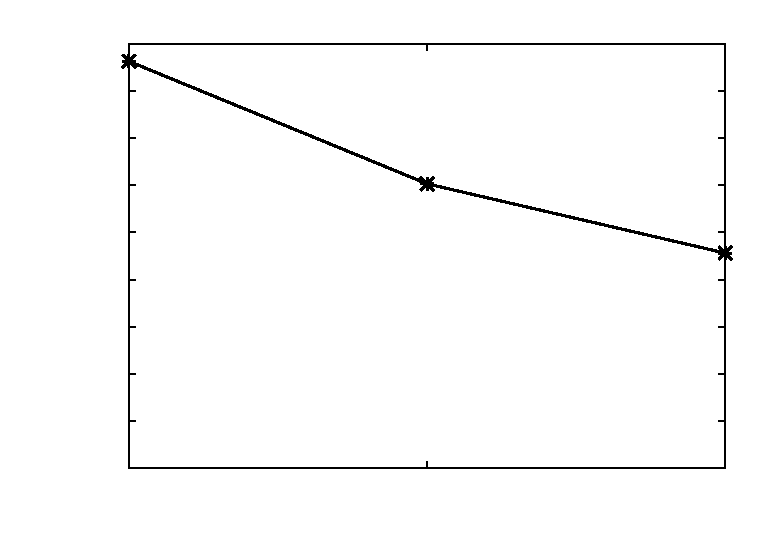
\includegraphics{graphs/clusters/grafico}}%
    \gplfronttext
  \end{picture}%
\endgroup
}
    \caption{Recovery period without new incoming requests}
    \label{fig:recovery_period}
\end{figure*}




\subsubsection{Restrain}\label{sec:eval:recovery:restrain}
%--------------------------------- Restrain --------------------------------- ---
%serial
We measured the duration of the restrain period considering two clients with a constant throughput of 400 requests/sec (Figure \ref{fig:restrain:serial}). 

Considering serial replay, the average response time of new incoming requests is 3.94\ms (95th percentile of 10.34\ms, 90th of 7.53\ms). Since the serial replay mode is not capable of fully exploring the application servers, the new incoming requests are not affected by the replay process. The replay process takes on average 30 minutes (1850\ms). Since the Shuttle takes 30 minutes to replay 1 million requests, the new flow generates 298 thousand new requests. Shuttle takes 18 minutes to replay these new requests. The user requests are suspended until the new requests are replayed and the branch is changed. This delay is considerable because the throughput of new requests is close to the throughput of the requests being replayed. The delay can be reduced by replaying the new requests and then block to replay the newer requests, i.e., creating several phases of replay. fazer varias fases, cada vez mais curtas porque vai compensando a diferenca. In addition, if the replay rate is bigger than the rate of new incoming requests, then the restrain phase is shorter.\\
%The serial replay mode is not capable of fully exploring the application servers so it takes almost one hour to recover (2953s total, 1100s in restrain mode) (Figure \ref{fig:restrain:serial})

%parallel
If Shuttle performs clustered replay, the application servers are overloaded. Consequently, the average response time of new incoming requests is 5.51\ms (95th percentile of 13.56\ms, 90th of 10.60\ms) and the throughput of the new incoming requests drops from 200 to 95 requests per second. On other hand, the throughput of requests being replayed drops from 1795 to 1686 req./sec. The recovery process takes a total 10 minutes (635 seconds). Therefore, the customers perform 56 000 requests. These requests are replayed in 46 seconds (Figure \ref{fig:restrain:clustered}). 



    
\begin{figure*}[!htb] 
    \centering
    \resizebox{0.7\linewidth}{!}{% GNUPLOT: LaTeX picture with Postscript
\begingroup
  \makeatletter
  \providecommand\color[2][]{%
    \GenericError{(gnuplot) \space\space\space\@spaces}{%
      Package color not loaded in conjunction with
      terminal option `colourtext'%
    }{See the gnuplot documentation for explanation.%
    }{Either use 'blacktext' in gnuplot or load the package
      color.sty in LaTeX.}%
    \renewcommand\color[2][]{}%
  }%
  \providecommand\includegraphics[2][]{%
    \GenericError{(gnuplot) \space\space\space\@spaces}{%
      Package graphicx or graphics not loaded%
    }{See the gnuplot documentation for explanation.%
    }{The gnuplot epslatex terminal needs graphicx.sty or graphics.sty.}%
    \renewcommand\includegraphics[2][]{}%
  }%
  \providecommand\rotatebox[2]{#2}%
  \@ifundefined{ifGPcolor}{%
    \newif\ifGPcolor
    \GPcolorfalse
  }{}%
  \@ifundefined{ifGPblacktext}{%
    \newif\ifGPblacktext
    \GPblacktexttrue
  }{}%
  % define a \g@addto@macro without @ in the name:
  \let\gplgaddtomacro\g@addto@macro
  % define empty templates for all commands taking text:
  \gdef\gplbacktext{}%
  \gdef\gplfronttext{}%
  \makeatother
  \ifGPblacktext
    % no textcolor at all
    \def\colorrgb#1{}%
    \def\colorgray#1{}%
  \else
    % gray or color?
    \ifGPcolor
      \def\colorrgb#1{\color[rgb]{#1}}%
      \def\colorgray#1{\color[gray]{#1}}%
      \expandafter\def\csname LTw\endcsname{\color{white}}%
      \expandafter\def\csname LTb\endcsname{\color{black}}%
      \expandafter\def\csname LTa\endcsname{\color{black}}%
      \expandafter\def\csname LT0\endcsname{\color[rgb]{1,0,0}}%
      \expandafter\def\csname LT1\endcsname{\color[rgb]{0,1,0}}%
      \expandafter\def\csname LT2\endcsname{\color[rgb]{0,0,1}}%
      \expandafter\def\csname LT3\endcsname{\color[rgb]{1,0,1}}%
      \expandafter\def\csname LT4\endcsname{\color[rgb]{0,1,1}}%
      \expandafter\def\csname LT5\endcsname{\color[rgb]{1,1,0}}%
      \expandafter\def\csname LT6\endcsname{\color[rgb]{0,0,0}}%
      \expandafter\def\csname LT7\endcsname{\color[rgb]{1,0.3,0}}%
      \expandafter\def\csname LT8\endcsname{\color[rgb]{0.5,0.5,0.5}}%
    \else
      % gray
      \def\colorrgb#1{\color{black}}%
      \def\colorgray#1{\color[gray]{#1}}%
      \expandafter\def\csname LTw\endcsname{\color{white}}%
      \expandafter\def\csname LTb\endcsname{\color{black}}%
      \expandafter\def\csname LTa\endcsname{\color{black}}%
      \expandafter\def\csname LT0\endcsname{\color{black}}%
      \expandafter\def\csname LT1\endcsname{\color{black}}%
      \expandafter\def\csname LT2\endcsname{\color{black}}%
      \expandafter\def\csname LT3\endcsname{\color{black}}%
      \expandafter\def\csname LT4\endcsname{\color{black}}%
      \expandafter\def\csname LT5\endcsname{\color{black}}%
      \expandafter\def\csname LT6\endcsname{\color{black}}%
      \expandafter\def\csname LT7\endcsname{\color{black}}%
      \expandafter\def\csname LT8\endcsname{\color{black}}%
    \fi
  \fi
  \setlength{\unitlength}{0.0500bp}%
  \begin{picture}(7200.00,5040.00)%
    \gplgaddtomacro\gplbacktext{%
      \csname LTb\endcsname%
      \put(1078,704){\makebox(0,0)[r]{\strut{} 0}}%
      \put(1078,1383){\makebox(0,0)[r]{\strut{} 500}}%
      \put(1078,2061){\makebox(0,0)[r]{\strut{} 1000}}%
      \put(1078,2740){\makebox(0,0)[r]{\strut{} 1500}}%
      \put(1078,3418){\makebox(0,0)[r]{\strut{} 2000}}%
      \put(1078,4097){\makebox(0,0)[r]{\strut{} 2500}}%
      \put(1078,4775){\makebox(0,0)[r]{\strut{} 3000}}%
      \put(1210,484){\makebox(0,0){\strut{}00:00}}%
      \put(1778,484){\makebox(0,0){\strut{}05:00}}%
      \put(2346,484){\makebox(0,0){\strut{}10:00}}%
      \put(2915,484){\makebox(0,0){\strut{}15:00}}%
      \put(3483,484){\makebox(0,0){\strut{}20:00}}%
      \put(4051,484){\makebox(0,0){\strut{}25:00}}%
      \put(4619,484){\makebox(0,0){\strut{}30:00}}%
      \put(5187,484){\makebox(0,0){\strut{}35:00}}%
      \put(5756,484){\makebox(0,0){\strut{}40:00}}%
      \put(6324,484){\makebox(0,0){\strut{}45:00}}%
      \put(176,2739){\rotatebox{-270}{\makebox(0,0){\strut{}Requests per second}}}%
      \put(4006,154){\makebox(0,0){\strut{}Time (minutes:seconds)}}%
      \put(4714,3418){\makebox(0,0)[l]{\strut{}Restrain}}%
    }%
    \gplgaddtomacro\gplfronttext{%
      \csname LTb\endcsname%
      \put(5816,4481){\makebox(0,0)[r]{\strut{}serial replay}}%
      \csname LTb\endcsname%
      \put(5816,4195){\makebox(0,0)[r]{\strut{}concurrent client}}%
    }%
    \gplbacktext
    \put(0,0){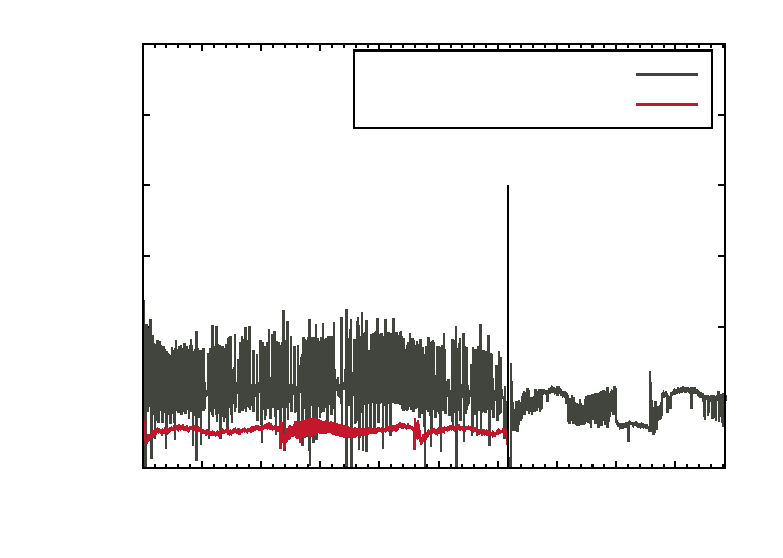
\includegraphics{graphs/restrain/serial_restrain}}%
    \gplfronttext
  \end{picture}%
\endgroup
}
    \caption{Serial Recovery: Requests throughput during the recovery period}
    \label{fig:restrain:serial}
\end{figure*}
    
\begin{figure*}[!htb] 
    \centering
    \resizebox{0.7\linewidth}{!}{% GNUPLOT: LaTeX picture with Postscript
\begingroup
  \makeatletter
  \providecommand\color[2][]{%
    \GenericError{(gnuplot) \space\space\space\@spaces}{%
      Package color not loaded in conjunction with
      terminal option `colourtext'%
    }{See the gnuplot documentation for explanation.%
    }{Either use 'blacktext' in gnuplot or load the package
      color.sty in LaTeX.}%
    \renewcommand\color[2][]{}%
  }%
  \providecommand\includegraphics[2][]{%
    \GenericError{(gnuplot) \space\space\space\@spaces}{%
      Package graphicx or graphics not loaded%
    }{See the gnuplot documentation for explanation.%
    }{The gnuplot epslatex terminal needs graphicx.sty or graphics.sty.}%
    \renewcommand\includegraphics[2][]{}%
  }%
  \providecommand\rotatebox[2]{#2}%
  \@ifundefined{ifGPcolor}{%
    \newif\ifGPcolor
    \GPcolorfalse
  }{}%
  \@ifundefined{ifGPblacktext}{%
    \newif\ifGPblacktext
    \GPblacktexttrue
  }{}%
  % define a \g@addto@macro without @ in the name:
  \let\gplgaddtomacro\g@addto@macro
  % define empty templates for all commands taking text:
  \gdef\gplbacktext{}%
  \gdef\gplfronttext{}%
  \makeatother
  \ifGPblacktext
    % no textcolor at all
    \def\colorrgb#1{}%
    \def\colorgray#1{}%
  \else
    % gray or color?
    \ifGPcolor
      \def\colorrgb#1{\color[rgb]{#1}}%
      \def\colorgray#1{\color[gray]{#1}}%
      \expandafter\def\csname LTw\endcsname{\color{white}}%
      \expandafter\def\csname LTb\endcsname{\color{black}}%
      \expandafter\def\csname LTa\endcsname{\color{black}}%
      \expandafter\def\csname LT0\endcsname{\color[rgb]{1,0,0}}%
      \expandafter\def\csname LT1\endcsname{\color[rgb]{0,1,0}}%
      \expandafter\def\csname LT2\endcsname{\color[rgb]{0,0,1}}%
      \expandafter\def\csname LT3\endcsname{\color[rgb]{1,0,1}}%
      \expandafter\def\csname LT4\endcsname{\color[rgb]{0,1,1}}%
      \expandafter\def\csname LT5\endcsname{\color[rgb]{1,1,0}}%
      \expandafter\def\csname LT6\endcsname{\color[rgb]{0,0,0}}%
      \expandafter\def\csname LT7\endcsname{\color[rgb]{1,0.3,0}}%
      \expandafter\def\csname LT8\endcsname{\color[rgb]{0.5,0.5,0.5}}%
    \else
      % gray
      \def\colorrgb#1{\color{black}}%
      \def\colorgray#1{\color[gray]{#1}}%
      \expandafter\def\csname LTw\endcsname{\color{white}}%
      \expandafter\def\csname LTb\endcsname{\color{black}}%
      \expandafter\def\csname LTa\endcsname{\color{black}}%
      \expandafter\def\csname LT0\endcsname{\color{black}}%
      \expandafter\def\csname LT1\endcsname{\color{black}}%
      \expandafter\def\csname LT2\endcsname{\color{black}}%
      \expandafter\def\csname LT3\endcsname{\color{black}}%
      \expandafter\def\csname LT4\endcsname{\color{black}}%
      \expandafter\def\csname LT5\endcsname{\color{black}}%
      \expandafter\def\csname LT6\endcsname{\color{black}}%
      \expandafter\def\csname LT7\endcsname{\color{black}}%
      \expandafter\def\csname LT8\endcsname{\color{black}}%
    \fi
  \fi
  \setlength{\unitlength}{0.0500bp}%
  \begin{picture}(7200.00,5040.00)%
    \gplgaddtomacro\gplbacktext{%
      \csname LTb\endcsname%
      \put(1078,704){\makebox(0,0)[r]{\strut{} 0}}%
      \put(1078,1383){\makebox(0,0)[r]{\strut{} 500}}%
      \put(1078,2061){\makebox(0,0)[r]{\strut{} 1000}}%
      \put(1078,2740){\makebox(0,0)[r]{\strut{} 1500}}%
      \put(1078,3418){\makebox(0,0)[r]{\strut{} 2000}}%
      \put(1078,4097){\makebox(0,0)[r]{\strut{} 2500}}%
      \put(1078,4775){\makebox(0,0)[r]{\strut{} 3000}}%
      \put(1210,484){\makebox(0,0){\strut{}00:00}}%
      \put(2267,484){\makebox(0,0){\strut{}02:00}}%
      \put(3324,484){\makebox(0,0){\strut{}04:00}}%
      \put(4381,484){\makebox(0,0){\strut{}06:00}}%
      \put(5438,484){\makebox(0,0){\strut{}08:00}}%
      \put(6495,484){\makebox(0,0){\strut{}10:00}}%
      \put(176,2739){\rotatebox{-270}{\makebox(0,0){\strut{}Requests per second}}}%
      \put(4006,154){\makebox(0,0){\strut{}Time (minutes:seconds)}}%
      \put(17505,3418){\makebox(0,0)[l]{\strut{}Restrain}}%
    }%
    \gplgaddtomacro\gplfronttext{%
      \csname LTb\endcsname%
      \put(5816,4481){\makebox(0,0)[r]{\strut{}clustered replay}}%
      \csname LTb\endcsname%
      \put(5816,4195){\makebox(0,0)[r]{\strut{}concurrent client}}%
    }%
    \gplbacktext
    \put(0,0){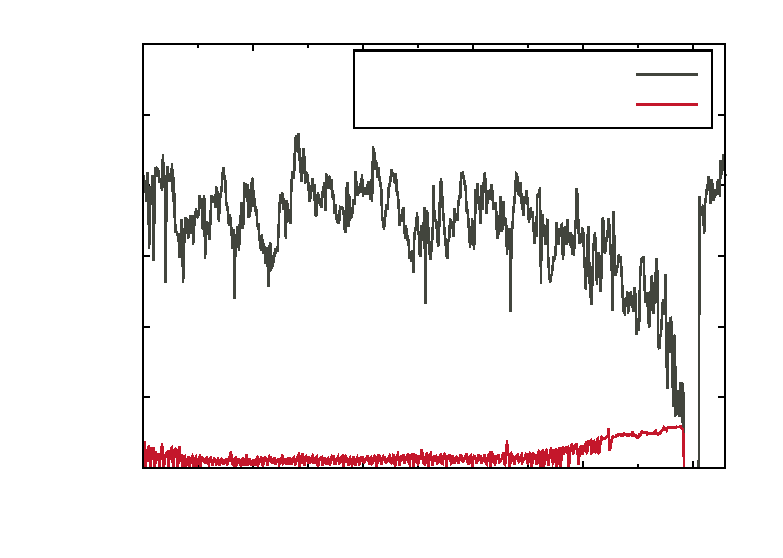
\includegraphics{graphs/restrain/clustered_restrain}}%
    \gplfronttext
  \end{picture}%
\endgroup
}
    \caption{Clustered Recovery: Requests throughput during the recovery period}
    \label{fig:restrain:clustered}
\end{figure*}


When a new application server is added, the throughput of the requests being replayed rises from 1686 to 2517 requests per second (397 seconds to recover), while the response latency to new requests is 4.61\ms. Therefore, we prove that adding more servers to perform replay allows to keep the quality of service for the customers.


%---------------------------------- replay instance ----------------------------------
%Qual o throughput maximo que uma replay instance consegue obter quando invoca directamente o application instance? Dificil de medir porque o application instance acaba por ser a limitacao quase sempre.
%The new requests are performed on new compute nodes. The \ac{HTTP} clients of each \textit{replay node} can perform \hl{XXX} request per second, using \hl{XXX} threads. (grafico a comparar com o numero de threads?)



%----------------------------------  scalability -------------------------------------
\subsubsection{Scalability}\label{sec:eval:recovery:scalability}
We measured how Shuttle leverages the horizontal scalability (adding more instances) of \ac{PaaS} to reduce the recovery period. We added \emph{c3.large} instances c3.large (7 \ac{ECU}s, 2 vCPUs, 2.8 GHz, Intel Xeon E5-2680v2, 3.75 GiB memory, 2 x 16 GiB Storage Capacity). The application server \emph{c3.xlarge} instance was downgraded to \emph{c3.large}. 

%serial
The serial replay with 2 application servers and 1 database takes 1347 seconds, while with 2 application servers an 2 database instances takes 1303 seconds (Figure \ref{fig:scalability:serial}). At larger scale, considering 2 databases, 6 application servers and 2 Shuttle storage instances, the process takes 1745\ms. Therefore, due to its implementation, the serial replay does not scale well. All instances remain with low resource usage. We expect to do much better by rewriting the implementation of the serial replay in the replay instances.

\begin{figure*}[!htb] 
    \centering
    \resizebox{0.6\linewidth}{!}{% GNUPLOT: LaTeX picture with Postscript
\begingroup
  \makeatletter
  \providecommand\color[2][]{%
    \GenericError{(gnuplot) \space\space\space\@spaces}{%
      Package color not loaded in conjunction with
      terminal option `colourtext'%
    }{See the gnuplot documentation for explanation.%
    }{Either use 'blacktext' in gnuplot or load the package
      color.sty in LaTeX.}%
    \renewcommand\color[2][]{}%
  }%
  \providecommand\includegraphics[2][]{%
    \GenericError{(gnuplot) \space\space\space\@spaces}{%
      Package graphicx or graphics not loaded%
    }{See the gnuplot documentation for explanation.%
    }{The gnuplot epslatex terminal needs graphicx.sty or graphics.sty.}%
    \renewcommand\includegraphics[2][]{}%
  }%
  \providecommand\rotatebox[2]{#2}%
  \@ifundefined{ifGPcolor}{%
    \newif\ifGPcolor
    \GPcolorfalse
  }{}%
  \@ifundefined{ifGPblacktext}{%
    \newif\ifGPblacktext
    \GPblacktexttrue
  }{}%
  % define a \g@addto@macro without @ in the name:
  \let\gplgaddtomacro\g@addto@macro
  % define empty templates for all commands taking text:
  \gdef\gplbacktext{}%
  \gdef\gplfronttext{}%
  \makeatother
  \ifGPblacktext
    % no textcolor at all
    \def\colorrgb#1{}%
    \def\colorgray#1{}%
  \else
    % gray or color?
    \ifGPcolor
      \def\colorrgb#1{\color[rgb]{#1}}%
      \def\colorgray#1{\color[gray]{#1}}%
      \expandafter\def\csname LTw\endcsname{\color{white}}%
      \expandafter\def\csname LTb\endcsname{\color{black}}%
      \expandafter\def\csname LTa\endcsname{\color{black}}%
      \expandafter\def\csname LT0\endcsname{\color[rgb]{1,0,0}}%
      \expandafter\def\csname LT1\endcsname{\color[rgb]{0,1,0}}%
      \expandafter\def\csname LT2\endcsname{\color[rgb]{0,0,1}}%
      \expandafter\def\csname LT3\endcsname{\color[rgb]{1,0,1}}%
      \expandafter\def\csname LT4\endcsname{\color[rgb]{0,1,1}}%
      \expandafter\def\csname LT5\endcsname{\color[rgb]{1,1,0}}%
      \expandafter\def\csname LT6\endcsname{\color[rgb]{0,0,0}}%
      \expandafter\def\csname LT7\endcsname{\color[rgb]{1,0.3,0}}%
      \expandafter\def\csname LT8\endcsname{\color[rgb]{0.5,0.5,0.5}}%
    \else
      % gray
      \def\colorrgb#1{\color{black}}%
      \def\colorgray#1{\color[gray]{#1}}%
      \expandafter\def\csname LTw\endcsname{\color{white}}%
      \expandafter\def\csname LTb\endcsname{\color{black}}%
      \expandafter\def\csname LTa\endcsname{\color{black}}%
      \expandafter\def\csname LT0\endcsname{\color{black}}%
      \expandafter\def\csname LT1\endcsname{\color{black}}%
      \expandafter\def\csname LT2\endcsname{\color{black}}%
      \expandafter\def\csname LT3\endcsname{\color{black}}%
      \expandafter\def\csname LT4\endcsname{\color{black}}%
      \expandafter\def\csname LT5\endcsname{\color{black}}%
      \expandafter\def\csname LT6\endcsname{\color{black}}%
      \expandafter\def\csname LT7\endcsname{\color{black}}%
      \expandafter\def\csname LT8\endcsname{\color{black}}%
    \fi
  \fi
  \setlength{\unitlength}{0.0500bp}%
  \begin{picture}(7200.00,5040.00)%
    \gplgaddtomacro\gplbacktext{%
      \csname LTb\endcsname%
      \put(1078,704){\makebox(0,0)[r]{\strut{} 0}}%
      \put(1078,1383){\makebox(0,0)[r]{\strut{} 500}}%
      \put(1078,2061){\makebox(0,0)[r]{\strut{} 1000}}%
      \put(1078,2740){\makebox(0,0)[r]{\strut{} 1500}}%
      \put(1078,3418){\makebox(0,0)[r]{\strut{} 2000}}%
      \put(1078,4097){\makebox(0,0)[r]{\strut{} 2500}}%
      \put(1078,4775){\makebox(0,0)[r]{\strut{} 3000}}%
      \put(1210,484){\makebox(0,0){\strut{}00:00}}%
      \put(1778,484){\makebox(0,0){\strut{}05:00}}%
      \put(2346,484){\makebox(0,0){\strut{}10:00}}%
      \put(2915,484){\makebox(0,0){\strut{}15:00}}%
      \put(3483,484){\makebox(0,0){\strut{}20:00}}%
      \put(4051,484){\makebox(0,0){\strut{}25:00}}%
      \put(4619,484){\makebox(0,0){\strut{}30:00}}%
      \put(5187,484){\makebox(0,0){\strut{}35:00}}%
      \put(5756,484){\makebox(0,0){\strut{}40:00}}%
      \put(6324,484){\makebox(0,0){\strut{}45:00}}%
      \put(176,2739){\rotatebox{-270}{\makebox(0,0){\strut{}Requests per second}}}%
      \put(4006,154){\makebox(0,0){\strut{}Time (minutes:seconds)}}%
      \put(4714,3418){\makebox(0,0)[l]{\strut{}Restrain}}%
    }%
    \gplgaddtomacro\gplfronttext{%
      \csname LTb\endcsname%
      \put(5816,4481){\makebox(0,0)[r]{\strut{}graphs/restrain/graphs/restrain/graphs/restrain/graphs/restrain/graphs/restrain/graphs/restrain/serial replay}}%
      \csname LTb\endcsname%
      \put(5816,4195){\makebox(0,0)[r]{\strut{}concurrent client}}%
    }%
    \gplbacktext
    \put(0,0){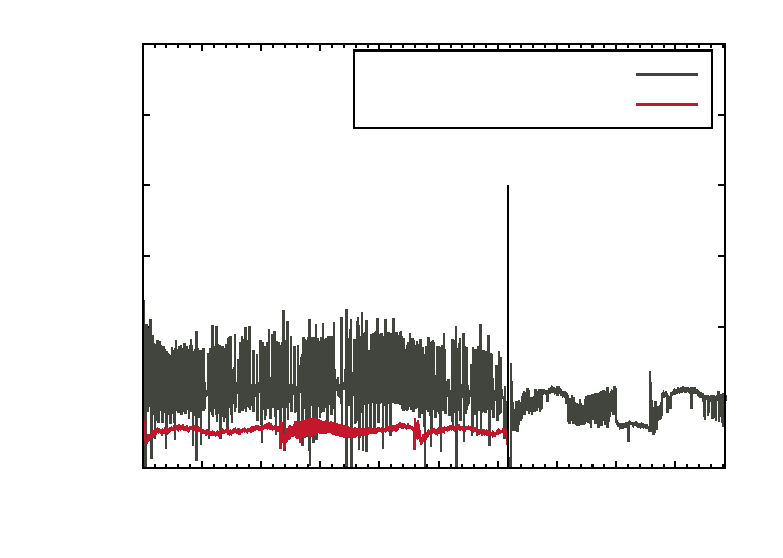
\includegraphics{graphs/restrain/graphs/restrain/graphs/restrain/graphs/restrain/graphs/restrain/graphs/restrain/graphs/restrain/serial}}%
    \gplfronttext
  \end{picture}%
\endgroup
}
    \caption{Shuttle Scalability Serial}
    \label{fig:scalability:serial}
\end{figure*}


%parallel
The Figure \ref{fig:scalability} (detailed values in Appendix \ref{appendix:results}) shows the recovery time using clustered replay. The figure demonstrates that Shuttle is scalable, in the sense that adding more servers allow reducing the time of recovery. Three application servers allowed recovery in half the time of one (750 versus 417 seconds). If the application runs on 5 or more application servers, then the single Shuttle Storage (Cassandra) instance becomes the bottleneck because Shuttle database client interceptor fetches the keys accessed by every request. We added another \emph{c3.xlarge} instance to the Cassandra cluster. 
\hl{reler esta seccao toda}
The latency of the requests during their first execution remains approximately constant when 3 servers are added (Figure \ref{fig:recovery_scalability:latency}). This means that a single \emph{TryOut} instance performing 2000 requests per second is not capable of overstraining the resources of the application servers.

\begin{figure*}[!htb]
  \centering
  \subfloat[][Recovery time (Clustered replay)]{
      \resizebox{0.5\linewidth}{!}{% GNUPLOT: LaTeX picture with Postscript
\begingroup
  \makeatletter
  \providecommand\color[2][]{%
    \GenericError{(gnuplot) \space\space\space\@spaces}{%
      Package color not loaded in conjunction with
      terminal option `colourtext'%
    }{See the gnuplot documentation for explanation.%
    }{Either use 'blacktext' in gnuplot or load the package
      color.sty in LaTeX.}%
    \renewcommand\color[2][]{}%
  }%
  \providecommand\includegraphics[2][]{%
    \GenericError{(gnuplot) \space\space\space\@spaces}{%
      Package graphicx or graphics not loaded%
    }{See the gnuplot documentation for explanation.%
    }{The gnuplot epslatex terminal needs graphicx.sty or graphics.sty.}%
    \renewcommand\includegraphics[2][]{}%
  }%
  \providecommand\rotatebox[2]{#2}%
  \@ifundefined{ifGPcolor}{%
    \newif\ifGPcolor
    \GPcolorfalse
  }{}%
  \@ifundefined{ifGPblacktext}{%
    \newif\ifGPblacktext
    \GPblacktexttrue
  }{}%
  % define a \g@addto@macro without @ in the name:
  \let\gplgaddtomacro\g@addto@macro
  % define empty templates for all commands taking text:
  \gdef\gplbacktext{}%
  \gdef\gplfronttext{}%
  \makeatother
  \ifGPblacktext
    % no textcolor at all
    \def\colorrgb#1{}%
    \def\colorgray#1{}%
  \else
    % gray or color?
    \ifGPcolor
      \def\colorrgb#1{\color[rgb]{#1}}%
      \def\colorgray#1{\color[gray]{#1}}%
      \expandafter\def\csname LTw\endcsname{\color{white}}%
      \expandafter\def\csname LTb\endcsname{\color{black}}%
      \expandafter\def\csname LTa\endcsname{\color{black}}%
      \expandafter\def\csname LT0\endcsname{\color[rgb]{1,0,0}}%
      \expandafter\def\csname LT1\endcsname{\color[rgb]{0,1,0}}%
      \expandafter\def\csname LT2\endcsname{\color[rgb]{0,0,1}}%
      \expandafter\def\csname LT3\endcsname{\color[rgb]{1,0,1}}%
      \expandafter\def\csname LT4\endcsname{\color[rgb]{0,1,1}}%
      \expandafter\def\csname LT5\endcsname{\color[rgb]{1,1,0}}%
      \expandafter\def\csname LT6\endcsname{\color[rgb]{0,0,0}}%
      \expandafter\def\csname LT7\endcsname{\color[rgb]{1,0.3,0}}%
      \expandafter\def\csname LT8\endcsname{\color[rgb]{0.5,0.5,0.5}}%
    \else
      % gray
      \def\colorrgb#1{\color{black}}%
      \def\colorgray#1{\color[gray]{#1}}%
      \expandafter\def\csname LTw\endcsname{\color{white}}%
      \expandafter\def\csname LTb\endcsname{\color{black}}%
      \expandafter\def\csname LTa\endcsname{\color{black}}%
      \expandafter\def\csname LT0\endcsname{\color{black}}%
      \expandafter\def\csname LT1\endcsname{\color{black}}%
      \expandafter\def\csname LT2\endcsname{\color{black}}%
      \expandafter\def\csname LT3\endcsname{\color{black}}%
      \expandafter\def\csname LT4\endcsname{\color{black}}%
      \expandafter\def\csname LT5\endcsname{\color{black}}%
      \expandafter\def\csname LT6\endcsname{\color{black}}%
      \expandafter\def\csname LT7\endcsname{\color{black}}%
      \expandafter\def\csname LT8\endcsname{\color{black}}%
    \fi
  \fi
  \setlength{\unitlength}{0.0500bp}%
  \begin{picture}(7200.00,5040.00)%
    \gplgaddtomacro\gplbacktext{%
      \csname LTb\endcsname%
      \put(946,704){\makebox(0,0)[r]{\strut{} 0}}%
      \put(946,1156){\makebox(0,0)[r]{\strut{} 100}}%
      \put(946,1609){\makebox(0,0)[r]{\strut{} 200}}%
      \put(946,2061){\makebox(0,0)[r]{\strut{} 300}}%
      \put(946,2513){\makebox(0,0)[r]{\strut{} 400}}%
      \put(946,2966){\makebox(0,0)[r]{\strut{} 500}}%
      \put(946,3418){\makebox(0,0)[r]{\strut{} 600}}%
      \put(946,3870){\makebox(0,0)[r]{\strut{} 700}}%
      \put(946,4323){\makebox(0,0)[r]{\strut{} 800}}%
      \put(946,4775){\makebox(0,0)[r]{\strut{} 900}}%
      \put(1078,484){\makebox(0,0){\strut{} 0}}%
      \put(1896,484){\makebox(0,0){\strut{} 1}}%
      \put(2714,484){\makebox(0,0){\strut{} 2}}%
      \put(3532,484){\makebox(0,0){\strut{} 3}}%
      \put(4349,484){\makebox(0,0){\strut{} 4}}%
      \put(5167,484){\makebox(0,0){\strut{} 5}}%
      \put(5985,484){\makebox(0,0){\strut{} 6}}%
      \put(6803,484){\makebox(0,0){\strut{} 7}}%
      \put(176,2739){\rotatebox{-270}{\makebox(0,0){\strut{}Time to recovery (seconds)}}}%
      \put(3940,154){\makebox(0,0){\strut{}Number of application servers}}%
    }%
    \gplgaddtomacro\gplfronttext{%
      \csname LTb\endcsname%
      \put(5816,4481){\makebox(0,0)[r]{\strut{}1 replay and 1 DB instance}}%
    }%
    \gplbacktext
    \put(0,0){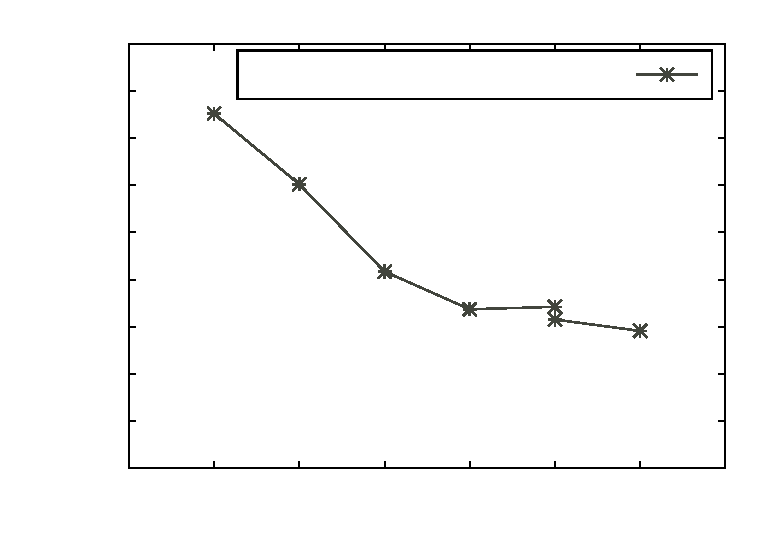
\includegraphics{graphs/scalability/recovery_time}}%
    \gplfronttext
  \end{picture}%
\endgroup
\label{fig:recovery_scalability}}
  } 
  \subfloat[][Response latency on first execution]{
      \resizebox{0.5\linewidth}{!}{% GNUPLOT: LaTeX picture with Postscript
\begingroup
  \makeatletter
  \providecommand\color[2][]{%
    \GenericError{(gnuplot) \space\space\space\@spaces}{%
      Package color not loaded in conjunction with
      terminal option `colourtext'%
    }{See the gnuplot documentation for explanation.%
    }{Either use 'blacktext' in gnuplot or load the package
      color.sty in LaTeX.}%
    \renewcommand\color[2][]{}%
  }%
  \providecommand\includegraphics[2][]{%
    \GenericError{(gnuplot) \space\space\space\@spaces}{%
      Package graphicx or graphics not loaded%
    }{See the gnuplot documentation for explanation.%
    }{The gnuplot epslatex terminal needs graphicx.sty or graphics.sty.}%
    \renewcommand\includegraphics[2][]{}%
  }%
  \providecommand\rotatebox[2]{#2}%
  \@ifundefined{ifGPcolor}{%
    \newif\ifGPcolor
    \GPcolorfalse
  }{}%
  \@ifundefined{ifGPblacktext}{%
    \newif\ifGPblacktext
    \GPblacktexttrue
  }{}%
  % define a \g@addto@macro without @ in the name:
  \let\gplgaddtomacro\g@addto@macro
  % define empty templates for all commands taking text:
  \gdef\gplbacktext{}%
  \gdef\gplfronttext{}%
  \makeatother
  \ifGPblacktext
    % no textcolor at all
    \def\colorrgb#1{}%
    \def\colorgray#1{}%
  \else
    % gray or color?
    \ifGPcolor
      \def\colorrgb#1{\color[rgb]{#1}}%
      \def\colorgray#1{\color[gray]{#1}}%
      \expandafter\def\csname LTw\endcsname{\color{white}}%
      \expandafter\def\csname LTb\endcsname{\color{black}}%
      \expandafter\def\csname LTa\endcsname{\color{black}}%
      \expandafter\def\csname LT0\endcsname{\color[rgb]{1,0,0}}%
      \expandafter\def\csname LT1\endcsname{\color[rgb]{0,1,0}}%
      \expandafter\def\csname LT2\endcsname{\color[rgb]{0,0,1}}%
      \expandafter\def\csname LT3\endcsname{\color[rgb]{1,0,1}}%
      \expandafter\def\csname LT4\endcsname{\color[rgb]{0,1,1}}%
      \expandafter\def\csname LT5\endcsname{\color[rgb]{1,1,0}}%
      \expandafter\def\csname LT6\endcsname{\color[rgb]{0,0,0}}%
      \expandafter\def\csname LT7\endcsname{\color[rgb]{1,0.3,0}}%
      \expandafter\def\csname LT8\endcsname{\color[rgb]{0.5,0.5,0.5}}%
    \else
      % gray
      \def\colorrgb#1{\color{black}}%
      \def\colorgray#1{\color[gray]{#1}}%
      \expandafter\def\csname LTw\endcsname{\color{white}}%
      \expandafter\def\csname LTb\endcsname{\color{black}}%
      \expandafter\def\csname LTa\endcsname{\color{black}}%
      \expandafter\def\csname LT0\endcsname{\color{black}}%
      \expandafter\def\csname LT1\endcsname{\color{black}}%
      \expandafter\def\csname LT2\endcsname{\color{black}}%
      \expandafter\def\csname LT3\endcsname{\color{black}}%
      \expandafter\def\csname LT4\endcsname{\color{black}}%
      \expandafter\def\csname LT5\endcsname{\color{black}}%
      \expandafter\def\csname LT6\endcsname{\color{black}}%
      \expandafter\def\csname LT7\endcsname{\color{black}}%
      \expandafter\def\csname LT8\endcsname{\color{black}}%
    \fi
  \fi
  \setlength{\unitlength}{0.0500bp}%
  \begin{picture}(7200.00,5040.00)%
    \gplgaddtomacro\gplbacktext{%
      \csname LTb\endcsname%
      \put(814,704){\makebox(0,0)[r]{\strut{} 0}}%
      \put(814,1383){\makebox(0,0)[r]{\strut{} 5}}%
      \put(814,2061){\makebox(0,0)[r]{\strut{} 10}}%
      \put(814,2740){\makebox(0,0)[r]{\strut{} 15}}%
      \put(814,3418){\makebox(0,0)[r]{\strut{} 20}}%
      \put(814,4097){\makebox(0,0)[r]{\strut{} 25}}%
      \put(814,4775){\makebox(0,0)[r]{\strut{} 30}}%
      \put(946,484){\makebox(0,0){\strut{} 0}}%
      \put(1783,484){\makebox(0,0){\strut{} 1}}%
      \put(2619,484){\makebox(0,0){\strut{} 2}}%
      \put(3456,484){\makebox(0,0){\strut{} 3}}%
      \put(4293,484){\makebox(0,0){\strut{} 4}}%
      \put(5130,484){\makebox(0,0){\strut{} 5}}%
      \put(5966,484){\makebox(0,0){\strut{} 6}}%
      \put(6803,484){\makebox(0,0){\strut{} 7}}%
      \put(176,2739){\rotatebox{-270}{\makebox(0,0){\strut{}Request latency (ms)}}}%
      \put(3874,154){\makebox(0,0){\strut{}Number of servers}}%
    }%
    \gplgaddtomacro\gplfronttext{%
      \csname LTb\endcsname%
      \put(5816,4481){\makebox(0,0)[r]{\strut{}1 replay and 1 DB instance}}%
    }%
    \gplbacktext
    \put(0,0){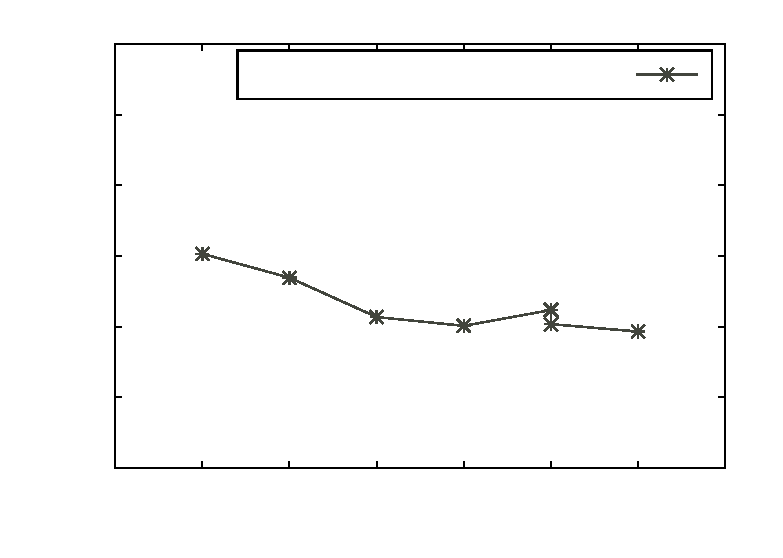
\includegraphics{graphs/scalability/latencia}}%
    \gplfronttext
  \end{picture}%
\endgroup
\label{fig:recovery_scalability:latency}}
  } 
  \caption{Shuttle Scalability}
  \label{fig:scalability}
\end{figure*}

When using less than 6 application servers, adding more database instances or clients does not improve the performance. When supporting 3 application servers, the \ac{CPU} usage of Voldemort database remains at 10\% on average. The \ac{CPU} usage of the instances that contain Shuttle's modules remains low (Figure \ref{fig:scalability:cpu:shuttle}). The bottleneck is the \ac{CPU} usage on the application servers (Figure \ref{fig:scalability:cpu:app}).

\begin{figure*}[!htb]
  \centering
  \subfloat[][CPU usage of Shuttle's instances ]{
      \resizebox{0.5\linewidth}{!}{% GNUPLOT: LaTeX picture with Postscript
\begingroup
  \makeatletter
  \providecommand\color[2][]{%
    \GenericError{(gnuplot) \space\space\space\@spaces}{%
      Package color not loaded in conjunction with
      terminal option `colourtext'%
    }{See the gnuplot documentation for explanation.%
    }{Either use 'blacktext' in gnuplot or load the package
      color.sty in LaTeX.}%
    \renewcommand\color[2][]{}%
  }%
  \providecommand\includegraphics[2][]{%
    \GenericError{(gnuplot) \space\space\space\@spaces}{%
      Package graphicx or graphics not loaded%
    }{See the gnuplot documentation for explanation.%
    }{The gnuplot epslatex terminal needs graphicx.sty or graphics.sty.}%
    \renewcommand\includegraphics[2][]{}%
  }%
  \providecommand\rotatebox[2]{#2}%
  \@ifundefined{ifGPcolor}{%
    \newif\ifGPcolor
    \GPcolorfalse
  }{}%
  \@ifundefined{ifGPblacktext}{%
    \newif\ifGPblacktext
    \GPblacktexttrue
  }{}%
  % define a \g@addto@macro without @ in the name:
  \let\gplgaddtomacro\g@addto@macro
  % define empty templates for all commands taking text:
  \gdef\gplbacktext{}%
  \gdef\gplfronttext{}%
  \makeatother
  \ifGPblacktext
    % no textcolor at all
    \def\colorrgb#1{}%
    \def\colorgray#1{}%
  \else
    % gray or color?
    \ifGPcolor
      \def\colorrgb#1{\color[rgb]{#1}}%
      \def\colorgray#1{\color[gray]{#1}}%
      \expandafter\def\csname LTw\endcsname{\color{white}}%
      \expandafter\def\csname LTb\endcsname{\color{black}}%
      \expandafter\def\csname LTa\endcsname{\color{black}}%
      \expandafter\def\csname LT0\endcsname{\color[rgb]{1,0,0}}%
      \expandafter\def\csname LT1\endcsname{\color[rgb]{0,1,0}}%
      \expandafter\def\csname LT2\endcsname{\color[rgb]{0,0,1}}%
      \expandafter\def\csname LT3\endcsname{\color[rgb]{1,0,1}}%
      \expandafter\def\csname LT4\endcsname{\color[rgb]{0,1,1}}%
      \expandafter\def\csname LT5\endcsname{\color[rgb]{1,1,0}}%
      \expandafter\def\csname LT6\endcsname{\color[rgb]{0,0,0}}%
      \expandafter\def\csname LT7\endcsname{\color[rgb]{1,0.3,0}}%
      \expandafter\def\csname LT8\endcsname{\color[rgb]{0.5,0.5,0.5}}%
    \else
      % gray
      \def\colorrgb#1{\color{black}}%
      \def\colorgray#1{\color[gray]{#1}}%
      \expandafter\def\csname LTw\endcsname{\color{white}}%
      \expandafter\def\csname LTb\endcsname{\color{black}}%
      \expandafter\def\csname LTa\endcsname{\color{black}}%
      \expandafter\def\csname LT0\endcsname{\color{black}}%
      \expandafter\def\csname LT1\endcsname{\color{black}}%
      \expandafter\def\csname LT2\endcsname{\color{black}}%
      \expandafter\def\csname LT3\endcsname{\color{black}}%
      \expandafter\def\csname LT4\endcsname{\color{black}}%
      \expandafter\def\csname LT5\endcsname{\color{black}}%
      \expandafter\def\csname LT6\endcsname{\color{black}}%
      \expandafter\def\csname LT7\endcsname{\color{black}}%
      \expandafter\def\csname LT8\endcsname{\color{black}}%
    \fi
  \fi
  \setlength{\unitlength}{0.0500bp}%
  \begin{picture}(7200.00,5040.00)%
    \gplgaddtomacro\gplbacktext{%
      \csname LTb\endcsname%
      \put(946,704){\makebox(0,0)[r]{\strut{} 0}}%
      \put(946,1111){\makebox(0,0)[r]{\strut{} 10}}%
      \put(946,1518){\makebox(0,0)[r]{\strut{} 20}}%
      \put(946,1925){\makebox(0,0)[r]{\strut{} 30}}%
      \put(946,2332){\makebox(0,0)[r]{\strut{} 40}}%
      \put(946,2740){\makebox(0,0)[r]{\strut{} 50}}%
      \put(946,3147){\makebox(0,0)[r]{\strut{} 60}}%
      \put(946,3554){\makebox(0,0)[r]{\strut{} 70}}%
      \put(946,3961){\makebox(0,0)[r]{\strut{} 80}}%
      \put(946,4368){\makebox(0,0)[r]{\strut{} 90}}%
      \put(946,4775){\makebox(0,0)[r]{\strut{} 100}}%
      \put(1078,484){\makebox(0,0){\strut{}00:00}}%
      \put(2223,484){\makebox(0,0){\strut{}02:00}}%
      \put(3368,484){\makebox(0,0){\strut{}04:00}}%
      \put(4513,484){\makebox(0,0){\strut{}06:00}}%
      \put(5658,484){\makebox(0,0){\strut{}08:00}}%
      \put(6803,484){\makebox(0,0){\strut{}10:00}}%
      \put(176,2739){\rotatebox{-270}{\makebox(0,0){\strut{}Maximum CPU Utilization (\%)}}}%
      \put(3940,154){\makebox(0,0){\strut{}Time (Hour:Minute)}}%
    }%
    \gplgaddtomacro\gplfronttext{%
      \csname LTb\endcsname%
      \put(5816,4481){\makebox(0,0)[r]{\strut{}HA Proxy + Proxy}}%
      \csname LTb\endcsname%
      \put(5816,4195){\makebox(0,0)[r]{\strut{}Replay Instance I + TryOut}}%
      \csname LTb\endcsname%
      \put(5816,3909){\makebox(0,0)[r]{\strut{}Manager + Cassandra I + Replay II}}%
    }%
    \gplbacktext
    \put(0,0){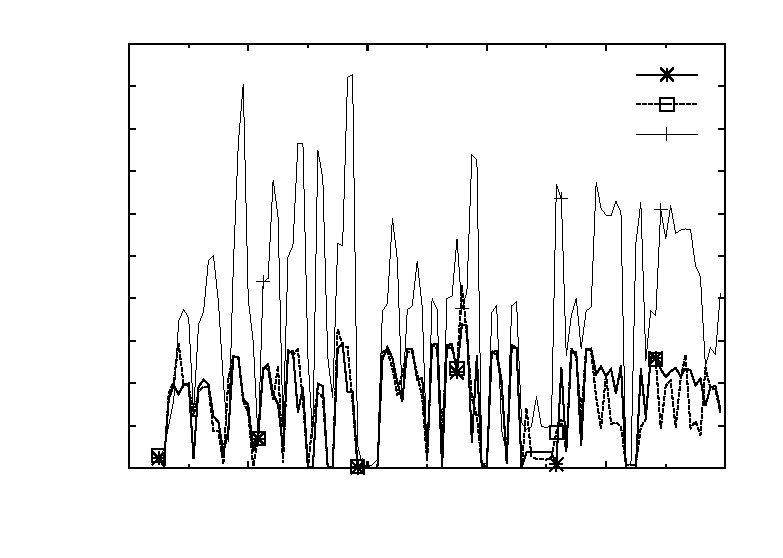
\includegraphics{graphs/usage/cpu_shuttle}}%
    \gplfronttext
  \end{picture}%
\endgroup
\label{fig:scalability:cpu:shuttle}}
  } 
  \subfloat[][CPU usage of Application instances ]{
      \resizebox{0.5\linewidth}{!}{% GNUPLOT: LaTeX picture with Postscript
\begingroup
  \makeatletter
  \providecommand\color[2][]{%
    \GenericError{(gnuplot) \space\space\space\@spaces}{%
      Package color not loaded in conjunction with
      terminal option `colourtext'%
    }{See the gnuplot documentation for explanation.%
    }{Either use 'blacktext' in gnuplot or load the package
      color.sty in LaTeX.}%
    \renewcommand\color[2][]{}%
  }%
  \providecommand\includegraphics[2][]{%
    \GenericError{(gnuplot) \space\space\space\@spaces}{%
      Package graphicx or graphics not loaded%
    }{See the gnuplot documentation for explanation.%
    }{The gnuplot epslatex terminal needs graphicx.sty or graphics.sty.}%
    \renewcommand\includegraphics[2][]{}%
  }%
  \providecommand\rotatebox[2]{#2}%
  \@ifundefined{ifGPcolor}{%
    \newif\ifGPcolor
    \GPcolorfalse
  }{}%
  \@ifundefined{ifGPblacktext}{%
    \newif\ifGPblacktext
    \GPblacktexttrue
  }{}%
  % define a \g@addto@macro without @ in the name:
  \let\gplgaddtomacro\g@addto@macro
  % define empty templates for all commands taking text:
  \gdef\gplbacktext{}%
  \gdef\gplfronttext{}%
  \makeatother
  \ifGPblacktext
    % no textcolor at all
    \def\colorrgb#1{}%
    \def\colorgray#1{}%
  \else
    % gray or color?
    \ifGPcolor
      \def\colorrgb#1{\color[rgb]{#1}}%
      \def\colorgray#1{\color[gray]{#1}}%
      \expandafter\def\csname LTw\endcsname{\color{white}}%
      \expandafter\def\csname LTb\endcsname{\color{black}}%
      \expandafter\def\csname LTa\endcsname{\color{black}}%
      \expandafter\def\csname LT0\endcsname{\color[rgb]{1,0,0}}%
      \expandafter\def\csname LT1\endcsname{\color[rgb]{0,1,0}}%
      \expandafter\def\csname LT2\endcsname{\color[rgb]{0,0,1}}%
      \expandafter\def\csname LT3\endcsname{\color[rgb]{1,0,1}}%
      \expandafter\def\csname LT4\endcsname{\color[rgb]{0,1,1}}%
      \expandafter\def\csname LT5\endcsname{\color[rgb]{1,1,0}}%
      \expandafter\def\csname LT6\endcsname{\color[rgb]{0,0,0}}%
      \expandafter\def\csname LT7\endcsname{\color[rgb]{1,0.3,0}}%
      \expandafter\def\csname LT8\endcsname{\color[rgb]{0.5,0.5,0.5}}%
    \else
      % gray
      \def\colorrgb#1{\color{black}}%
      \def\colorgray#1{\color[gray]{#1}}%
      \expandafter\def\csname LTw\endcsname{\color{white}}%
      \expandafter\def\csname LTb\endcsname{\color{black}}%
      \expandafter\def\csname LTa\endcsname{\color{black}}%
      \expandafter\def\csname LT0\endcsname{\color{black}}%
      \expandafter\def\csname LT1\endcsname{\color{black}}%
      \expandafter\def\csname LT2\endcsname{\color{black}}%
      \expandafter\def\csname LT3\endcsname{\color{black}}%
      \expandafter\def\csname LT4\endcsname{\color{black}}%
      \expandafter\def\csname LT5\endcsname{\color{black}}%
      \expandafter\def\csname LT6\endcsname{\color{black}}%
      \expandafter\def\csname LT7\endcsname{\color{black}}%
      \expandafter\def\csname LT8\endcsname{\color{black}}%
    \fi
  \fi
  \setlength{\unitlength}{0.0500bp}%
  \begin{picture}(7200.00,5040.00)%
    \gplgaddtomacro\gplbacktext{%
      \csname LTb\endcsname%
      \put(946,704){\makebox(0,0)[r]{\strut{} 0}}%
      \put(946,1518){\makebox(0,0)[r]{\strut{} 20}}%
      \put(946,2332){\makebox(0,0)[r]{\strut{} 40}}%
      \put(946,3147){\makebox(0,0)[r]{\strut{} 60}}%
      \put(946,3961){\makebox(0,0)[r]{\strut{} 80}}%
      \put(946,4775){\makebox(0,0)[r]{\strut{} 100}}%
      \put(1078,484){\makebox(0,0){\strut{}00:00}}%
      \put(1894,484){\makebox(0,0){\strut{}02:00}}%
      \put(2709,484){\makebox(0,0){\strut{}04:00}}%
      \put(3525,484){\makebox(0,0){\strut{}06:00}}%
      \put(4340,484){\makebox(0,0){\strut{}08:00}}%
      \put(5156,484){\makebox(0,0){\strut{}10:00}}%
      \put(176,2739){\rotatebox{-270}{\makebox(0,0){\strut{}Maximum CPU Utilization (\%)}}}%
      \put(3117,154){\makebox(0,0){\strut{}Time (Hour:Minute)}}%
    }%
    \gplgaddtomacro\gplfronttext{%
      \csname LTb\endcsname%
      \put(6212,4544){\makebox(0,0)[r]{\strut{}Server II }}%
      \csname LTb\endcsname%
      \put(6212,4258){\makebox(0,0)[r]{\strut{}Server III }}%
      \csname LTb\endcsname%
      \put(6212,3972){\makebox(0,0)[r]{\strut{}Server IV }}%
      \csname LTb\endcsname%
      \put(6212,3686){\makebox(0,0)[r]{\strut{}Server V }}%
      \csname LTb\endcsname%
      \put(6212,3400){\makebox(0,0)[r]{\strut{}Server VI }}%
    }%
    \gplbacktext
    \put(0,0){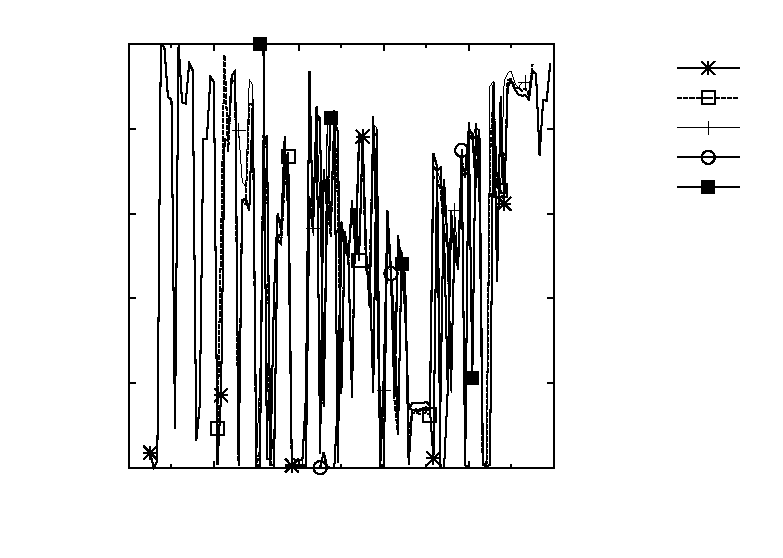
\includegraphics{graphs/usage/cpu_app}}%
    \gplfronttext
  \end{picture}%
\endgroup
\label{fig:scalability:cpu:app}}
  } 
  \caption{CPU Usage during several execution and replay phases}
  \label{fig:scalability:cpu}
\end{figure*}

%In \emph{Ask}, the voting requests represent 4\% of the total number of requests. These requests only increment a variable. Incrementar uma variavel ate 1000 implica 1000 requests enquanto que saber o seu valor e fazer set a 1000 implicaria apenas 1 request.

We conclude the application servers to be the main performance harm. The performance of the application servers can be improved. If application developers for \ac{PaaS} optimize their applications to execute more requests per unit of time, then the recovery period is reduced. %Shuttle's scalability depends on its algorithms and implementation
Most of \ac{PaaS} controller watch the load of the instances. One area of future development is to dynamically adapt the throughput of the replay instances to the load of the application and database instances.



%If a new database instance is added, then the delay is \hl{xxxx} and the throughput of the replaying requests is \hl{xxxx}.
%The recovery period varies with the dependencies between requests. Shuttle reduces the recovery period by replaying independent clusters in parallel. 
% \begin{figure*}[!htb]
%     \resizebox{0.5\linewidth}{!}{% GNUPLOT: LaTeX picture with Postscript
\begingroup
  \makeatletter
  \providecommand\color[2][]{%
    \GenericError{(gnuplot) \space\space\space\@spaces}{%
      Package color not loaded in conjunction with
      terminal option `colourtext'%
    }{See the gnuplot documentation for explanation.%
    }{Either use 'blacktext' in gnuplot or load the package
      color.sty in LaTeX.}%
    \renewcommand\color[2][]{}%
  }%
  \providecommand\includegraphics[2][]{%
    \GenericError{(gnuplot) \space\space\space\@spaces}{%
      Package graphicx or graphics not loaded%
    }{See the gnuplot documentation for explanation.%
    }{The gnuplot epslatex terminal needs graphicx.sty or graphics.sty.}%
    \renewcommand\includegraphics[2][]{}%
  }%
  \providecommand\rotatebox[2]{#2}%
  \@ifundefined{ifGPcolor}{%
    \newif\ifGPcolor
    \GPcolorfalse
  }{}%
  \@ifundefined{ifGPblacktext}{%
    \newif\ifGPblacktext
    \GPblacktexttrue
  }{}%
  % define a \g@addto@macro without @ in the name:
  \let\gplgaddtomacro\g@addto@macro
  % define empty templates for all commands taking text:
  \gdef\gplbacktext{}%
  \gdef\gplfronttext{}%
  \makeatother
  \ifGPblacktext
    % no textcolor at all
    \def\colorrgb#1{}%
    \def\colorgray#1{}%
  \else
    % gray or color?
    \ifGPcolor
      \def\colorrgb#1{\color[rgb]{#1}}%
      \def\colorgray#1{\color[gray]{#1}}%
      \expandafter\def\csname LTw\endcsname{\color{white}}%
      \expandafter\def\csname LTb\endcsname{\color{black}}%
      \expandafter\def\csname LTa\endcsname{\color{black}}%
      \expandafter\def\csname LT0\endcsname{\color[rgb]{1,0,0}}%
      \expandafter\def\csname LT1\endcsname{\color[rgb]{0,1,0}}%
      \expandafter\def\csname LT2\endcsname{\color[rgb]{0,0,1}}%
      \expandafter\def\csname LT3\endcsname{\color[rgb]{1,0,1}}%
      \expandafter\def\csname LT4\endcsname{\color[rgb]{0,1,1}}%
      \expandafter\def\csname LT5\endcsname{\color[rgb]{1,1,0}}%
      \expandafter\def\csname LT6\endcsname{\color[rgb]{0,0,0}}%
      \expandafter\def\csname LT7\endcsname{\color[rgb]{1,0.3,0}}%
      \expandafter\def\csname LT8\endcsname{\color[rgb]{0.5,0.5,0.5}}%
    \else
      % gray
      \def\colorrgb#1{\color{black}}%
      \def\colorgray#1{\color[gray]{#1}}%
      \expandafter\def\csname LTw\endcsname{\color{white}}%
      \expandafter\def\csname LTb\endcsname{\color{black}}%
      \expandafter\def\csname LTa\endcsname{\color{black}}%
      \expandafter\def\csname LT0\endcsname{\color{black}}%
      \expandafter\def\csname LT1\endcsname{\color{black}}%
      \expandafter\def\csname LT2\endcsname{\color{black}}%
      \expandafter\def\csname LT3\endcsname{\color{black}}%
      \expandafter\def\csname LT4\endcsname{\color{black}}%
      \expandafter\def\csname LT5\endcsname{\color{black}}%
      \expandafter\def\csname LT6\endcsname{\color{black}}%
      \expandafter\def\csname LT7\endcsname{\color{black}}%
      \expandafter\def\csname LT8\endcsname{\color{black}}%
    \fi
  \fi
  \setlength{\unitlength}{0.0500bp}%
  \begin{picture}(7200.00,5040.00)%
    \gplgaddtomacro\gplbacktext{%
      \csname LTb\endcsname%
      \put(1078,704){\makebox(0,0)[r]{\strut{} 20}}%
      \put(1078,1518){\makebox(0,0)[r]{\strut{} 20.2}}%
      \put(1078,2332){\makebox(0,0)[r]{\strut{} 20.4}}%
      \put(1078,3147){\makebox(0,0)[r]{\strut{} 20.6}}%
      \put(1078,3961){\makebox(0,0)[r]{\strut{} 20.8}}%
      \put(1078,4775){\makebox(0,0)[r]{\strut{} 21}}%
      \put(1210,484){\makebox(0,0){\strut{} 0}}%
      \put(2142,484){\makebox(0,0){\strut{} 2}}%
      \put(3074,484){\makebox(0,0){\strut{} 4}}%
      \put(4007,484){\makebox(0,0){\strut{} 6}}%
      \put(4939,484){\makebox(0,0){\strut{} 8}}%
      \put(5871,484){\makebox(0,0){\strut{} 10}}%
      \put(6803,484){\makebox(0,0){\strut{} 12}}%
      \put(176,2739){\rotatebox{-270}{\makebox(0,0){\strut{}Recovery time (ms)}}}%
      \put(4006,154){\makebox(0,0){\strut{}Number of requests}}%
    }%
    \gplgaddtomacro\gplfronttext{%
      \csname LTb\endcsname%
      \put(5816,4602){\makebox(0,0)[r]{\strut{}1 Cluster}}%
      \csname LTb\endcsname%
      \put(5816,4382){\makebox(0,0)[r]{\strut{}2 Clusters}}%
      \csname LTb\endcsname%
      \put(5816,4162){\makebox(0,0)[r]{\strut{}3 Cluster}}%
      \csname LTb\endcsname%
      \put(5816,3942){\makebox(0,0)[r]{\strut{}4 Clusters}}%
      \csname LTb\endcsname%
      \put(5816,3722){\makebox(0,0)[r]{\strut{}5 Clusters}}%
    }%
    \gplbacktext
    \put(0,0){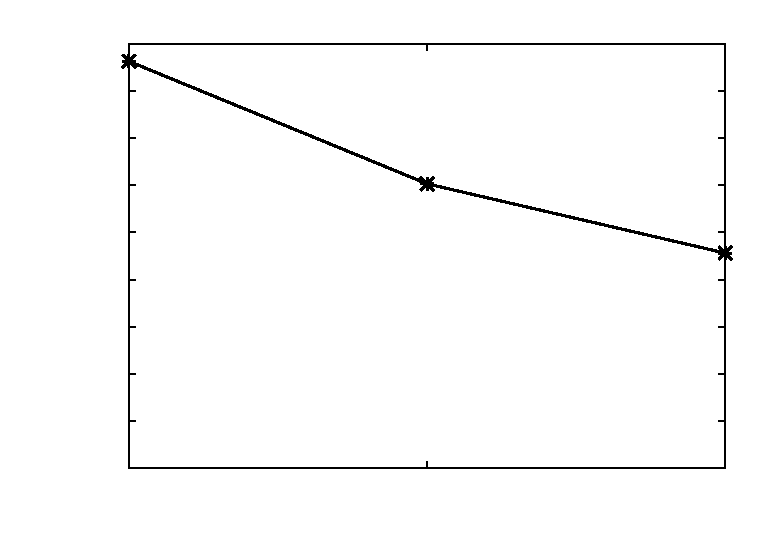
\includegraphics{graphs/clusters/grafico}}%
    \gplfronttext
  \end{picture}%
\endgroup
}
%     \caption{\textbf{Clustering influence on recovery time: throughput vs clustering: 1 cluster, 10 clusters, 100 clusters, 1000 clusters, 10000 clusters}}
%     \label{fig:clustering_influence}
% \end{figure*}


%%%%%%%%%%%%%%%%%%%%%%%%%%%%%%%%%%%%%%%%%%%%%%%%%%%%%%%%%%%%%%%%%%%%%%%%%%%%%%%%%%%%%%%%%%%%%%%%%%%%%%%%%%%%%%%%
\subsection{Space Overhead}\label{sec:eval:storage}
The storage overhead is relevant because it is a payed cloud resource and Shuttle stores every user request. The space overhead is defined by the variables in Table \ref{tab:storage_variables}.

\begin{table}[ht]
\centering
\begin{tabular}{l|ll}
\textbf{Module}          & \textbf{Contains}      & \textbf{Depends on}    \\ \hline
\textbf{Shuttle Storage} &                        &                          \\
                         & Request                & request content          \\
                         & Response (optional)    & response content         \\
                         & Accessed keys          & key size and number of database operations per request\\
                         & Start and end instants & constant overhead           \\ \hline
\textbf{Database instance} &                      &                          \\
                          & Version list          & number of snapshots per data item \\
                          & Operation list        & number of operations per data item \\ \hline
\textbf{Dependency graph} &                       &                                   \\
                        & Dependencies            & number of dependencies per request\\
\end{tabular}
\caption{Variables on Shuttle's storage}
\label{tab:storage_variables}
\end{table}

Requests to static contents, e.g., images, are ignored. For instance, a question page of StackOverflow \cite{stackoverflow} implies 30 static content requests. Shuttle is not implemented for web-services with large requests, such has file hosting services, because the data would be duplicated in the requests and storage. Shuttle architecture would remain similar on those services but would require an algorithm to reduce the storage overhead by detecting duplicated data.\\

%define request size
Most of applications' requests, including headers, vary in size from 200 bytes to over 2KB, depending on the number of application cookies \cite{spdy}. As applications use more cookies and user agents expand features, typical header sizes of 700-800 bytes are common \cite{spdy}. Shuttle adds the \ac{SRD}, which has 35 bytes, to every request. Requests of \emph{Ask} based on the StackExchange Network have an average size of 216 bytes (std. def of 124 bytes, 95th percentile of 274 bytes,  99th of 494 bytes in a sample of 200 thousand requests, in which 95\% are read requests).

%shuttle storage
Requests and keys are stored in the \emph{Shuttle storage} (Cassandra) while the dependency graph and database operations are kept in  manager and database instances. Values at Table \ref{tab:storage_overhead} represent the size of each component in memory \footnote{https://code.google.com/p/memory-measurer} to store the workload, defined above (1 million requests, from which 95\% are requests to read a question). No snapshot has been taken and the data is not compressed.

\begin{table}[ht]
\centering
  \begin{tabular}{l|rr}   
              & \# objects   & size (total) (MB) \\ \hline
  \textbf{Shuttle Storage: }             \\
  Request     & 1 million    & 212       \\  %1000000 - 212 162 883
  Response    & 1 million    & 8 967     \\  %1000000 - 8 967 233 474 
  Start/End   & 2 million    & 16        \\  %2000000 - 16 000 000
  Keys        & 137 million  & 488       \\  %137 244 585  - 488 862 483
  Total       &              & 9 684     \\  %9 684258 840
  \textbf{Database node:} & 14 593 entries \\ 
  Version   List &  14 593    &  1.4       \\ %14 593 - 1 400 928   - 96 bytes
  Operation List &  9 million &  277       \\ %9 551 908 - 277 019 984   - 29 bytes
  Total       &               & 282 \\ %282 230 960
  \textbf{Manager:} & & \\ 
  Graph       & 1 million     & 718 \\  %718 486 432
  \end{tabular}            
\caption{Storage used by Shuttle}
\label{tab:storage_overhead}
\end{table}


%Cassandra
The start/end instants have a constant size of 16 bytes because each timestamp is a long. The size of the list of keys accessed by the request depends on the key length and the number of accesses. The request of the workload defined above represent 212 MBytes. The main overhead are the requests, as we are storing them complete (the full \ac{HTTP} pages). Notice that Shuttle has to store the responses only if the tenants use the \ac{API} to solve inconsistencies (Section \ref{sec:arch:consistency}). In addition, the size of the responses can be reduced if applications fetch only data using a \ac{REST} \ac{API} instead of the entire page.

Since \ac{HTTP} messages are similar, we evaluated how a compression technique can reduce the storage usage. While Cassandra stores 9GB of data, the compression algorithm of Cassandra, \emph{lz4} \cite{lz4}, reduces the size in disk to 4.9 GB (including Cassandra's metadata). For instance, considering an arrival rate of 1000 requests per second (86 million per day), a half-year (15.638 billion requests) requires 3.3 TB. 

%For instance, the algorithm \emph{lz4} can compress a text file with 1 million requests by \hl{xxxx} \% and \hl{xxxx} \% in \hl{xxxx} seconds. A ideia era colocar tudo em ficheiros e depois usar o algoritmo para comprimir e ver quanto da}\\


%database node
The snapshot mechanism requires to track a new version when a data item is written by the first time after a snapshot. Each version has 10 bytes. The overhead can be reduced implementing the version list as a bitmap. In addition, each database operation implies to store 13 bytes to record its \acf{RID} and type in the \emph{operation list}. The total database storage overhead encompasses synchronization mechanisms and object references. Notice that the storage and performance overhead can be distributed by several instances because the data items are independent. \\

%graph
The dependency graph is a double-linked graph implemented as a Hash Table. Each of its entries represents a request. It contains the start and end instants of the requests and two lists of \ac{RID}: requests to execute before, requests to execute after. Each entry in the Hash Table has, on average, 718 bytes bytes, and depends on 1 requests and 5 requests depend on it (Table \ref{tab:memory:depgrah}). The start and end instants has 32 bytes. Each dependency has 16 bytes. 

For the sake of performance in selective replay, the dependency graph is doubly-linked, a single-linked graph requires, on average, 458 bytes per entry. In order to reduce the storage overhead, a doubly-linked graph can be generated from a single-linked graph.


\begin{table}[ht]
\centering   
  \begin{tabular}{l|rr}     
           & \# objects & size (bytes) \\ \hline  
  Start    & 1          & 16           \\
  End      & 1          & 16           \\                        
  Before   & 1          & 61           \\     %   1 199 305 - 40 487 088 bytes for sample of 663 105 entries
  After    & 5          & 162          \\     % 153 356 416 -  3 527 873 bytes for sample of 663 105 entries
  Total    & -          & 718 MB       \\     % 718 486 432 -  1 000 000 entries
  \end{tabular}            
\caption{Memory used by each entry of dependency graph}
\label{tab:memory:depgrah}
\end{table}

%\hl{na tabela da memoria por entrada há erro porque o array é alocado em excesso}


Tenants can reduce the storage overhead removing old snapshots, operations and requests. However, they shall take into account that Shuttle needs a snapshot previous to the intrusion instant to recover the application.

In conclusion, the main storage overhead are the \ac{HTTP} responses. We propose several ways to reduce the storage overhead. Since the data stored by Shuttle is likely to be similar, compression techniques can reduce the storage overhead.



%%%%%%%%%%%%%%%%%%%%%%%%%%%%%%%%%%%%%%%%%%%%%%%%%%%%%%%%%%%%%%%%%%%%%%%%%%%%%%%%%%%%%%%%%%%%%%%%%%%%%%%%%%%%%%%%
\section{Monetary Cost}\label{sec:eval:cost}
We measured the monetary cost of the intrusion recovery process using a public cloud provider. The intrusion recovery costs are come from two sources: storage and computation resources. The following prices represent the current cost of \acf{AWS} in North Virgina.

We consider an execution of \emph{Ask} application with a constant arrival rate of 250 requests per second (20 million per day) and the storage usage defined in Section \ref{sec:eval:storage}. This is a common rate for an enterprise application, for instance the Portuguese Ministry of Finances (Table \ref{tab:base_throughputs}). We also define that Shuttle shall allow to recover from attacks that have occurred during the last 3 months. Therefore, Shuttle needs to store 2 billion requests. We assume that the recovery process re-executes 50 million requests, independent of the schema (full/serial replay). \\

Table \ref{tab:storageScale} represents the estimated storage overhead based on the measurements introduced in Section \ref{sec:eval:storage}. We do not consider Shuttle to store the responses.%aqui arredondei os numeros, há problema? perda de rigor cientifico? 

\begin{table}[ht]
\centering
\begin{tabular}{l|rrr}
                  & 1 million   & 20 million (day)    & 2 billion (quarter) \\ \hline
Shuttle Storage   & 716 MB      & 14.32 GB            & 1.432 TB \\
Graph             & 718 MB      & 14.36 GB            & 1.436 TB \\
Database Nodes    & 282 MB      &  5.64 GB            & 564 GB   \\
\end{tabular}
\caption{Storage overhead considering different number of stored requests}
\label{tab:storageScale}
\end{table}


%cost of request storage
The user requests can be stored in \acf{AWS} \ac{S3}, DynamoDB, Glacier and \acf{EBS} (Table \ref{tab:s3Cost}). \emph{S3} is a scalable object storage, \emph{EBS} block level storage, \emph{Glacier} low-cost storage service for data archiving and online backup, \emph{DynamoDB} low-latency \acs{NoSQL} database. Their usage costs are also distinct (Table \ref{tab:s3Cost:usage}).

 \begin{table}[h]
 \centering
 \begin{tabular}{l|rrrr}
 \multirow{2}{*}{Data per month} & \multicolumn{4}{c}{Cost  per GB-month} \\
                                 & S3         & Glacier   & EBS     & DynamoDB   \\ \hline
    First 1 TB                   & \$0.0300   & 0.0100    & 0.05    & 0.25 \\
    Next 49 TB                   & \$0.0295   & 0.0100    & 0.05    & 0.25 \\
    Next 450 TB                  & \$0.0290   & 0.0100    & 0.05    & 0.25 \\
    Next 500 TB                  & \$0.0285   & 0.0100    & 0.05    & 0.25 \\
    Next 4000 TB                 & \$0.0280   & 0.0100    & 0.05    & 0.25 \\
    Next 5000 TB                 & \$0.0275   & 0.0100    & 0.05    & 0.25 \\
    \end{tabular}
    \caption{Pricing of Amazon Web Services S3, Glacier, EBS and DynamoDB}
    \label{tab:s3Cost}
\end{table}


\begin{table}[ht]
\centering
\begin{tabular}{l|rrrr}
\multirow{2}{*}{\textbf{Operation}} & \multicolumn{4}{c}{\textbf{Usage cost per month}}                                          \\
                                    & \textbf{S3}     & \textbf{Glacier}                   & \textbf{EBS}  & \textbf{DynamoDB} \\ \hline
\textbf{Put}                        & 0.005 (1k ops)  & \multicolumn{1}{r}{0.050 (1k ops)} & 0.05 (1M ops) & 0.0065 (Hour)     \\
\textbf{Get}                        & 0.0004 (1k ops) & 0.01 (1 GB)                        & 0.05 (1M ops) & 0.0065 (Hour)    
\end{tabular}
\caption{Usage cost of Amazon Web Services S3, Glacier, \ac{EBS} and DynamoDB}
\label{tab:s3Cost:usage}
\end{table}


Glacier has the lowest cost to store data for long period but the highest per insert operation. In contrast, DynamoDB provides the lowest cost per insert operation, lower latency but the highest per stored gigabyte. The best storage model depends on the application usage pattern. We propose to store the most recent data in \emph{DynamoDB} and archive the data in periodically in \emph{Glacier}. We assume that the data in DynamoDB is archived every day, i.e., each batch stores a day.

%DynamoDB
Shuttle generates an average of 35 GB per day, which costs \$8.75 per month to store in DynamoDB. Considering a provisioned capacity of 36,000 writes per hour and 180,000 strongly consistent reads per hour, the DynamoDB usage costs \$4.83 per-month.

%Glacier
The Glacier stores 3.433 TB, which represents the archives of the latest quarter, so it costs \$34.33 per month. Since the daily backup can be compressed in a single file, the number of put requests per month is lower than 1 thousand so it costs less than \$0.05. Tenants can retrieve up to 5\% of average monthly storage for free. Since we consider an attack that taint 1 million requests, the required download of 2 GB is free. This data is loaded in DynamoDB to perform the replay process. 

In total, the storage overhead of Shuttle costs \$47 per month if the application retrieves 20 million requests per day.\\


% The DynamoDB pricing \cite{dynamoDB}, which Voldemort is based-on, is \$0.00735 per hour for every 10 units of Write Capacity (enough capacity to do up to 36,000 writes per hour) and \$0.00735 per hour for every 50 units of Read Capacity (enough capacity to do up to 180,000 strongly consistent reads, or 360,000 eventually consistent reads, per hour). The storage costs \$0.283 per GB-month, excluding the cost of a per-item storage overhead of 100 bytes to account for indexing. The data transfered to DynamoDB is free, while the data transfer out of Dynamo has the following cost (Table \ref{tab:dynamoCost}).
% \begin{table}
%   \centering
%    \begin{tabular}{|l|l|}
%     \hline
%     Data Transfer OUT per Month    & Cost per GB  \\ \hline
%    First 1GB   &  \$0.000 \\ \hline
%    Up to 10TB  &  \$0.120 \\ \hline
%    Next 40TB   &  \$0.090 \\ \hline
%    Next 100TB   & \$0.070 \\ \hline
%    Next 350TB   & \$0.050 \\ \hline
%     \end{tabular}
%     \caption{Pricing of Amazon Web Services DynamoDB Pricing}
%     \label{tab:dynamoCost}
% \end{table}

% Considering 30 million requests to submit a new question, which perform \hl{XXXX} reads and \hl{XXXX} writes. The DynamoDB most be increased \hl{XXX} units of Read Capacity and  \hl{XXX} units of Write Capacity. The cost of get the 30 million requests from \ac{S3} with aggregation of 1000 requests is \$0.012.



%cost of computation
Since Shuttle is designed to be integrated with the cloud provider infrastructure, namely the load balancer and the database, the costs of the database and proxy overhead are hard to predict. The Shuttle manager is also included in the underlying cloud provider infrastructure and can be shared by multiple clients. 

The Table \ref{tab:ec2Cost} represents the costs of the computation instances in \ac{AWS}. The data transfer between computing instances and the database is free in the same region using private \ac{IP} addresses.

In Section \ref{sec:eval:performance}, we demonstrate that Shuttle requires two extra \emph{c3.xlarge} instances: the manager and the proxy. To recover the application, Shuttle can replay 1 million requests in 400 seconds using 5 application servers (\emph{c3.large} instances) and 1 \emph{c3.xlarge} replay instance.

Considering a full-hour, these instances have an associated cost of \$1 per instance-hour, which means that Shuttle can replay 1 million requests by the cost of \$1. Since Shuttle allocating more instances reduces the recovery period, Shuttle leverages the elasticity and pay-per-usage model of cloud computing to provide a cost-efficient intrusion recovery solution. 

\begin{table}
  \centering
   \begin{tabular}{|l|r|r|r|r|r|}
\hline
            & \bf{vCPU} & \bf{ECU}    & \bf{Memory (GiB)}  & \bf{Instance Storage (GiB)}  & \bf{Cost per Hour } \\ \hline
t2.small    & 1         & Variable    & 2                  & EBS Only                     & \$0.028            \\ \hline
t2.medium   & 2         & Variable    & 4                  & EBS Only                     & \$0.056            \\ \hline
m3.medium   & 1         & 3           & 3.75               & 1x4 SSD                      & \$0.077            \\ \hline
m3.large    & 2         & 6.5         & 7.5                & 1x32 SSD                     & \$0.154            \\ \hline
m3.xlarge   & 4         & 13          & 15                 & 2x40 SSD                     & \$0.308            \\ \hline
m3.2xlarge  & 8         & 26          & 30                 & 2x80 SSD                     & \$0.616            \\ \hline
c3.large    & 2         & 7           & 3.75               & 2x16 SSD                     & \$0.120            \\ \hline
c3.xlarge   & 4         & 14          & 7.5                & 2x40 SSD                     & \$0.239            \\ \hline
c3.2xlarge  & 8         & 28          & 15                 & 2x80 SSD                     & \$0.478            \\ \hline
c3.4xlarge  & 16        & 55          & 30                 & 2x160 SSD                    & \$0.956            \\ \hline
c3.8xlarge  & 32        & 108         & 60                 & 2x320 SSD                    & \$1.912            \\ \hline
\end{tabular}
\caption{Pricing of Amazon Web Services \ac{EC2} Instances }
\label{tab:ec2Cost}
\end{table}

In conclusion, the cost of Shuttle is dominated by the storage because the replay instances are allocated on demand and paid-per usage.\\

Notice that the costs are estimations for the application prototype and vary with the type and usage of the tenants applications. In addition, Shuttle aims to be integrated as a service in the public \acf{CSP} infrastructure: the proxy is integrated into the load-balancer and the database proxy is integrated in the database instances. Each manager and Shuttle storage can be shared by several tenants. Therefore, we expect providers to define a pay-per-usage model of Shuttle service. In addition, providers can reduce the costs because the data stored by several tenants is similar thus can be compressed. We do not address the creation of a pay-per-usage model in this document but we would like to address it in our future research.

\subsection{Discussion}\label{sec:eval:performance:discussion}
In this section we measured the performance overhead, the duration and scalability of the recovery process, the storage requirements and the cost of the used resources. We evaluated Shuttle usage for the prototype application \emph{Ask}. Shuttle is designed to support various \ac{PaaS} applications with distinct semantics.

The evaluated metrics depend on several aspects of the application. Taking into account all that was mention, we identified the following factors to be the most relevant:

\begin{enumerate}
  \item Request rate
  \item Request/response size
  \item Detection delay
  \item Dependency between requests   
  \item Number of operations per request
\end{enumerate}                              

Clearly, much future research and development will be needed to create a version of Shuttle for web-scale applications. The performance of Shuttle modules can be optimized and tunned to archive better performance and lower storage footprint, reducing the costs and recovery period.

Nevertheless, we validated our single proxy architecture. The proxy imposes a throughput limitation but this limitation is acceptable for most of applications. Moreover, this limitation does not affect the recovery period.

We presented a cost estimation for Shuttle usage. In future, we expect to provide a generic pricing model that \acf{CSP} can use to provide Shuttle on a pay-per-usage manner.


%%%%%%%%%%%%%%%%%%%%%%%%%%%%%%%%%%%%%%%%%%%%%%%%%%%%%%%%%%%%%%%%%%%%%%%%%%%%%%%%%%%%%%%%%%%%%%%%%%%%%%%%%%%%%%%%
\section{Chapter Summary}\label{sec:eval:performance:summary}
The main conclusions of the Shuttle evaluation presented in this chapter are:
\begin{enumerate}
  \item The full replay has lower precision than selective replay but the recovery time is acceptable and allows to remove malicious actions not logged by the proxy.
  \item The prototype accuracy and performance is acceptable for small and enterprise applications.
  \item It is possible to duplicate the number of requests replayed per second by increasing the number of application servers from 1 to 3. 
  \item The main storage overhead is the response storage but the data can be compressed. 
  \item The usage cost of Shuttle is low considering its advantages.
\end{enumerate}          


%-------------------------------- EXCLUIDOS ---------------------------------------------------



% We measured the performance overhead considering three distinct system loads: real-world example, medium load and heavy load.
% %Real World
% The real world load consists on the simulation of the requests retrieved by the StackExchange.com from \hl{XXXXX} until \hl{XXXXX}, which corresponds to \hl{XXXXX} requests. Requests create \hl{XXX} questions, \hl{XXX} answers, \hl{XXX} comments and \hl{XXXX} votes. The tenant performs a weekly snapshot. The database size at begin of the experiment is \hl{XXXX} entries, \hl{XXX} GB.\\
% The attack is detected at 30 July 2013, 200 days after its occurrence at 10 January 2013.
% \textbf{Recovery:} The recovery process requires to replay \hl{XXXX} requests. .........................

% %Medium Throughput
% The medium load scenario simulates a constant request arrival rate of 4 requests per second (345 600 per day): one question, one answer, one comment and one vote. The tenant performs a daily snapshot.
% \textbf{Recovery:} The recovery process requires to replay \hl{XXXX} requests. .........................

% %High Throughput}
% The high throughput scenario simulates two request flows. The first with a constant request arrival rate of \hl{XXXX quantos requests pode ser visto como excelente?} requests per second (\hl{X} per day). The other flow has a request arrival rate of \hl{XXXX} request per second during 4 hours per day. The tenant performs a daily snapshot.
% \textbf{Recovery:} The recovery process requires to replay \hl{XXXX} requests. .........................
% (enough capacity to do up to 180,000 strongly consistent reads, or 360,000 eventually consistent reads, per hour)* ---> DynamoDB 50 units of Read
% (enough capacity to do up to 36,000 writes per hour) --> DynamoDB 10 units of Write
% Let’s assume that your application needs to perform 1 million writes and 1 million reads per day, while storing 3 GB of data. For simplicity, let’s assume that your workload is relatively constant throughout the day and your items are less than 1 KB in size. (You can easily scale up and down to deal with variable workloads and adjust for larger items, but for this example we’ll keep it simple).
% First, you need to calculate how many writes and reads per second you need. 1 million evenly spread writes per day is equivalent to 1,000,000 (writes) / 24 (hours) / 60 (minutes) / 60 (seconds) = 11.6 writes per second. A DynamoDB Write Capacity Unit can handle 1 write per second, so you need 12 Write Capacity Units. Similarly, to handle 1 million reads per day, you need 12 Read Capacity Units.







